%
% Template Laporan Skripsi/Thesis 
%
% @author  Andreas Febrian, Lia Sadita 
% @version 1.03
%
% Dokumen ini dibuat berdasarkan standar IEEE dalam membuat class untuk 
% LaTeX dan konfigurasi LaTeX yang digunakan Fahrurrozi Rahman ketika 
% membuat laporan skripsi. Konfigurasi yang lama telah disesuaikan dengan 
% aturan penulisan thesis yang dikeluarkan UI pada tahun 2008.
%

%
% Tipe dokumen adalah report dengan satu kolom. 
%
\documentclass[12pt, a4paper, onecolumn, oneside, final]{report}

% Load konfigurasi LaTeX untuk tipe laporan thesis
\usepackage{uithesis}
\usepackage{bm}
\usepackage[numbers]{natbib}
\usepackage{import}
\usepackage{hyperref}
\usepackage{xcolor}
% Load konfigurasi khusus untuk laporan yang sedang dibuat
%-----------------------------------------------------------------------------%
% Informasi Mengenai Dokumen
%-----------------------------------------------------------------------------%
% 
% Judul laporan. 
\var{\judul}{Judul Sesuatu Banget \f{English} Miring Juga}
% 
% Tulis kembali judul laporan, kali ini akan diubah menjadi huruf kapital
\Var{\Judul}{JUDUL SESUATU BANGET \f{ENGLISH} MIRING JUGA}
% 
% Tulis kembali judul laporan namun dengan bahasa Ingris
\var{\judulInggris}{Sesuatu Banget in English}

% 
% Tipe laporan, dapat berisi Skripsi, Tugas Akhir, Thesis, atau Disertasi
\var{\type}{Tugas Akhir}
% 
% Tulis kembali tipe laporan, kali ini akan diubah menjadi huruf kapital
\Var{\Type}{Tugas Akhir}
% 
% Tulis nama penulis 
\var{\penulis}{Tegar Aldina Galari}
% 
% Tulis kembali nama penulis, kali ini akan diubah menjadi huruf kapital
\Var{\Penulis}{Tegar Aldina Galari}
% 
% Tulis NPM penulis
\var{\npm}{1306407376}
% 
% Tuliskan Fakultas dimana penulis berada
\Var{\Fakultas}{Ilmu Komputer}
\var{\fakultas}{Ilmu Komputer}
% 
% Tuliskan Program Studi yang diambil penulis
\Var{\Program}{Ilmu Komputer}
\var{\program}{Ilmu Komputer }
\var{\programEng}{Computer Science}
% 
% Tuliskan tahun publikasi laporan
\Var{\bulanTahun}{Juli 2017}
% 
% Tuliskan gelar yang akan diperoleh dengan menyerahkan laporan ini
\var{\gelar}{Sarjana Ilmu Komputer}
% 
% Tuliskan tanggal pengesahan laporan, waktu dimana laporan diserahkan ke 
% penguji/sekretariat
\var{\tanggalPengesahan}{21 Juni 2013} 
% 
% Tuliskan tanggal keputusan sidang dikeluarkan dan penulis dinyatakan 
% lulus/tidak lulus
\var{\tanggalLulus}{5 Juli 2013}
% 
% Tuliskan pembimbing 
\var{\pembimbing}{Prof. Saya }
\var{\pembimbingdua}{Dia S.Kom, M.Kom}
%
% Tuliskan tempat anda kuliah
\var{\kampus}{Universitas Indonesia }
% 
% Alias untuk memudahkan alur penulisan paa saat menulis laporan
\var{\Saya}{Penulis }
\var{\saya}{penulis }

%-----------------------------------------------------------------------------%
% Judul Setiap Bab
%-----------------------------------------------------------------------------%
% 
% Berikut ada judul-judul setiap bab. 
% Silahkan diubah sesuai dengan kebutuhan. 
% 
\Var{\kataPengantar}{Kata Pengantar}
\Var{\babSatu}{Pendahuluan}
\Var{\babDua}{Landasan Teori}
\Var{\babTiga}{Metodologi Penelitian}
\Var{\babEmpat}{Perancangan Implementasi dan Analisis}
\Var{\babLima}{Implementasi dan Pengujian}
\Var{\babEnam}{Hasil Implementasi dan Evaluasi}
\Var{\babTujuh}{Kesimpulan dan Saran}

% Berikut singkatan singkatan yang sering digunakan
% Informasi teknologi asosiasi amerika
\var{\ITTA}{Information Technology Assiciation of America }

\var{\kemkominfo}{Kementrian Komunikasi dan Informasi }
\var{\game}{\textit{video game }}
\var{\ddp}{dasar dasar pemograman }
\var{\DDP}{Dasar dasar pemograman }
\var{\topik}{Iterator }
% Daftar pemenggalan suku kata dan istilah dalam LaTeX
%
% Hyphenation untuk Indonesia 
%
% @author  Andreas Febrian
% @version 1.00
% 
% Tambahkan cara pemenggalan kata-kata yang salah dipenggal secara otomatis 
% oleh LaTeX. Jika kata tersebut dapat dipenggal dengan benar, maka tidak 
% perlu ditambahkan dalam berkas ini. Tanda pemenggalan kata menggunakan 
% tanda '-'; contoh:
% menarik
%   --> pemenggalan: me-na-rik
%

\hyphenation{
    % alphabhet A
    a-na-li-sa a-tur 
    a-pli-ka-si 
    % alphabhet B
    ba-ngun-an 
    be-be-ra-pa 
    ber-ge-rak
    ber-ke-lan-jut-an 
    ber-pe-nga-ruh 
    % alphabhet C
    ca-ri
    % alphabhet D
    di-ban-ding-kan
    di-de-fi-ni-si-kan
    di-ha-rap-kan
    di-ka-te-go-ri-kan
    di-mi-li-ki-nya
    di-se-rah-kan
    di-sim-pan di-pim-pin de-ngan da-e-rah di-ba-ngun da-pat di-nya-ta-kan 
    di-sim-bol-kan di-pi-lih di-li-hat de-fi-ni-si
    di-se-su-ai-kan
    di-pi-sah-kan
    % alphabhet E
    e-le-men
    e-ner-gi eks-klu-sif
    % alphabhet F
    fa-si-li-tas
    % alphabhet G
    ga-bung-an ge-rak
    % alphabhet H
    ha-lang-an
    he-te-ro-gen
    % alphabhet I
    i-ngin
    % alphabhet J
    % alphabhet K
    ke-hi-lang-an
    ku-ning 
    kua-li-tas ka-me-ra ke-mung-kin-an ke-se-pa-ham-an
    ke-te-pat-an
    kon-fi-gu-ra-si
    % alphabhet L
    ling-kung-an
    % alphabhet M
    me-min-ta
    me-mo-del-kan
    me-mo-ri
    men-de-fi-ni-si-kan
    me-neng-ah
    meng-a-tas-i me-mung-kin-kan me-nge-na-i me-ngi-rim-kan 
    meng-u-bah meng-a-dap-ta-si me-nya-ta-kan mo-di-fi-ka-si
    meng-a-tur
    meng-au-to-ma-si
    meng-a-ko-mo-da-si
    me-ngo-rek-si
    me-nyim-pan
    % alphabhet N
    nya-ta non-eks-klu-sif
    % alphabhet O
    % alphabhet P
    pa-ra-lel
    peng-ala-mat-an
    pen-ting
    penga-da-an
	pe-nye-rap-an 
	pe-ngon-trol
    pe-mo-del-an
    pe-ran  pe-ran-an-nya
    pe-rin-tah
    pem-ba-ngun-an pre-si-den pe-me-rin-tah prio-ri-tas peng-am-bil-an 
    peng-ga-bung-an pe-nga-was-an pe-ngem-bang-an 
    pe-nga-ruh pa-ra-lel-is-me per-hi-tung-an per-ma-sa-lah-an 
    pen-ca-ri-an peng-struk-tur-an
    pe-ner-bang-an
    pro-se-sor
    % alphabhet Q
    % alphabhet R
    ran-cang-an
    % alphabhet S
    se-dang-kan
    se-ring
    si-mu-la-si sa-ngat    
    % alphabhet T
    te-ngah
    ter-da-pat
    % alphabhet U
    u-sa-ha
    % alphabhet V
    % alphabhet W
    % alphabhet X
    % alphabhet Y
    % alphabhet Z
    % special
}
% Daftar istilah yang mungkin perlu ditandai 
%
% @author  Andreas Febrian
% @version 1.00
% 
% Mendaftar seluruh istilah yang mungkin akan perlu dijadikan 
% italic atau bold pada setiap kemunculannya dalam dokumen. 
% 

\var{\license}{\f{Creative Common License 1.0 Generic}}
\var{\bslash}{$\setminus$}


%\usepackage[backend=bibtex]{biblatex}
%\addbibresource{bib.bib}

% Awal bagian penulisan laporan
\begin{document}
%
% Sampul Laporan
%
% Sampul Laporan

%
% @author  unknown
% @version 1.01
% @edit by Andreas Febrian
%

\begin{titlepage}
    \begin{center}    
        \begin{figure}
            \begin{center}
                
\includegraphics[width=2.5cm]{pics/makara.png}
            \end{center}
        \end{figure}    
        \vspace*{0cm}
        \bo{
        	UNIVERSITAS INDONESIA\\
        }
        
        \vspace*{1.0cm}
        % judul thesis harus dalam 14pt Times New Roman
        \bo{\Judul} \\[1.0cm]

        \vspace*{2.5 cm}    
        % harus dalam 14pt Times New Roman
        \bo{\Type}

        \vspace*{3 cm}       
        % penulis dan npm
        \bo{\Penulis} \\
        \bo{\npm} \\

        \vspace*{5.0cm}

        % informasi mengenai fakultas dan program studi
        \bo{
        	FAKULTAS \Fakultas\\
        	PROGRAM STUDI \Program \\
        	DEPOK \\
        	\bulanTahun
        }
    \end{center}
\end{titlepage}


%
% Gunakan penomeran romawi
\pagenumbering{roman}

%
% load halaman judul dalam
\addChapter{HALAMAN JUDUL}
%
% Halaman Judul Laporan 
%
% @author  unknown
% @version 1.01
% @edit by Andreas Febrian
%

\begin{titlepage}
    \begin{center}\begin{figure}
            \begin{center}
                
\includegraphics[width=2.5cm]{pics/makara.png}
            \end{center}
        \end{figure}    
        \vspace*{0cm}
        \bo{
        	UNIVERSITAS INDONESIA\\
        }
        
        \vspace*{1.0cm}
        % judul thesis harus dalam 14pt Times New Roman
        \bo{\Judul} \\[1.0cm]

        \vspace*{2.5 cm}    
        % harus dalam 14pt Times New Roman
        \bo{\Type} \\
        % keterangan prasyarat
        \bo{Diajukan sebagai salah satu syarat untuk memperoleh gelar \\
        \gelar}\\

        \vspace*{3 cm}       
        % penulis dan npm
        \bo{\Penulis} \\
        \bo{\npm} \\

        \vspace*{5.0cm}

        % informasi mengenai fakultas dan program studi
        \bo{
        	FAKULTAS \Fakultas\\
        	PROGRAM STUDI \Program \\
        	DEPOK \\
        	\bulanTahun
        }
    \end{center}
\end{titlepage}

%
% setelah bagian ini, halaman dihitung sebagai halaman ke 2
\setcounter{page}{2}

% sementara ga usah
% load halaman pengesahan
%\addChapter{LEMBAR PERSETUJUAN}
%%
% Halaman Pengesahan
%
% @author  Andreas Febrian
% @author  Ardhi Putra Pratama
% @version 1.1
%

\chapter*{HALAMAN PERSETUJUAN}

\vspace*{0.2cm}
\noindent 

\noindent
\begin{tabular}{l l p{11cm}}
	\bo{Judul}&: & \judul \\ 
	\bo{Nama}&: & \penulis \\
	\bo{NPM}&: & \npm \\
\end{tabular} \\

\vspace*{1.2cm}


\noindent\begin{minipage}[b]{0.6\hsize}
  \raggedright
  Laporan \type~ini telah diperiksa dan disetujui.\\[0.3cm]
  
  \tanggalPengesahan \\[2cm]
  
  \underline{\pembimbing}\\[0.1cm]
  Pembimbing \type
\end{minipage}
\hfill
\begin{minipage}[b]{0.4\hsize}
  \raggedleft
  .\\[2cm]
  \underline{\pembimbingdua}\\[0.1cm]
  Pembimbing \type
\end{minipage}

\newpage
%
% load halaman orisinalitas 
\addChapter{LEMBAR PERNYATAAN ORISINALITAS}
%
% Halaman Orisinalitas
%
% @author  Andreas Febrian
% @version 1.01
%

\chapter*{\uppercase{halaman pernyataan orisinalitas}}
\vspace*{2cm}

\begin{center}
	\bo{\type~ini adalah hasil karya saya sendiri, \\ 
	dan semua sumber baik yang dikutip maupun dirujuk \\
	telah saya nyatakan dengan benar.} \\
	\vspace*{2.6cm}
	
	\begin{tabular}{l c l}
	\bo{Nama} & : & \bo{\penulis} \\
	\bo{NPM} & : & \bo{\npm} \\ 
	\bo{Tanda Tangan} & : & \\
	& & \\
	& & \\
	\bo{Tanggal} & : & \bo{\tanggalPengesahan} \\	
	\end{tabular}
\end{center}

\newpage
%
%
\addChapter{LEMBAR PENGESAHAN}
%
% Halaman Pengesahan Sidang
%
% @author  Andreas Febrian, Andre Tampubolon 
% @version 1.02
%

\chapter*{HALAMAN PENGESAHAN}

\vspace*{0.4cm}
\noindent 

\noindent
\begin{tabular}{ll p{9cm}}
	\type~ini diajukan oleh&: & \\
	Nama&: & \penulis \\
	NPM&: & \npm \\
	Program Studi&: & \program \\
	Judul \type&: & \judul \\
\end{tabular} \\

\vspace*{1.0cm}

\noindent \bo{Telah berhasil dipertahankan di hadapan Dewan Penguji 
dan diterima sebagai bagian persyaratan yang diperlukan untuk 
memperoleh gelar \gelar~pada Program Studi \program, Fakultas 
\fakultas, Universitas Indonesia.}\\[0.2cm]

\begin{center}
	\bo{DEWAN PENGUJI}
\end{center}

\vspace*{0.3cm}

\begin{tabular}{l l l l }
	& & & \\
	Pembimbing&: & \pembimbing & (\hspace*{3.0cm}) \\
	& & & \\
	Pembimbing&: & \pembimbingdua & (\hspace*{3.0cm}) \\
	& & & \\
	Penguji&: & Drs. Lim Yohanes Stefanus M.Math., Ph.D. & (\hspace*{3.0cm}) \\
	& & & \\
	Penguji&: & Sauel Louvan, ST., M.Sc. & (\hspace*{3.0cm}) \\
\end{tabular}\\

\vspace*{2.0cm}

\begin{tabular}{ll l}
	Ditetapkan di&: & Depok\\
	Tanggal&: & \tanggalLulus \\
\end{tabular}


\newpage
%
%
\addChapter{\kataPengantar}
%-----------------------------------------------------------------------------%
\chapter*{\kataPengantar}
%-----------------------------------------------------------------------------%
\textcolor{red}{[MASIH DARI TEMPLATE]} \f{Alhamdulillahirabbil'alamin}, segala puji dan syukur kehadirat Tuhan Yang Maha Esa, Allah Subhana Huwataala, karena hanya dengan hidayah dan rahmat-Nya, penulis dapat menyelesaikan pembuatan skripsi ini.

\f{Allahumma sholli 'alaa sayyidina Muhammad}, Sholawat serta salam tak henti-hentinya dipanjatkan kepada Rasulullah SAW, atas peranannya di muka bumi dalam memberikan tuntunan kepada seluruh umat manusia, dan sebagai inspirasi atas seluruh manusia sebagai manusia dengan akhlak terbaik.

Penulisan skripsi ini ditujukan untuk memenuhi salah satu syarat untuk menyelesaikan pendidikan pada Program \gelar, Universitas Indonesia. Saya sadar bahwa dalam perjalanan menempuh kegiatan penerimaan dan adaptasi, belajar-mengajar, hingga penulisan skripsi ini, penulis tidak sendirian. Penulis ingin berterima kasih kepada pihak-pihak berikut : 

\vspace*{0.1cm}
\begin{flushright}
Depok, \tanggalPengesahan \\[0.1cm]
\vspace*{1cm}
\penulis

\end{flushright}
%
%
\addChapter{LEMBAR PERSETUJUAN PUBLIKASI ILMIAH}
% 
% @author  Andre Tampubolon, Andreas Febrian
% @version 1.01
% 

\chapter*{\uppercase{Halaman Pernyataan Persetujuan Publikasi Tugas Akhir untuk Kepentingan Akademis}}

\vspace*{0.2cm}
\noindent 
Sebagai sivitas akademik Universitas Indonesia, saya yang bertanda 
tangan di bawah ini:
\vspace*{0.4cm}


\begin{tabular}{p{4.2cm} l p{6cm}}
	\bo{Nama} & : & \penulis \\ 	
	\bo{NPM} & : & \npm \\
	\bo{Program Studi} & : & \program\\	
	\bo{Fakultas} & : & \fakultas\\
	\bo{Jenis Karya} & : & \type \\
\end{tabular}

\vspace*{0.6cm}
\noindent demi pengembangan ilmu pengetahuan, menyetujui untuk memberikan 
kepada Universitas Indonesia \bo{Hak Bebas Royalti Noneksklusif 
(Non-exclusive Royalty Free Right)} atas karya ilmiah saya yang berjudul:
\begin{center}
	\judul
\end{center}
beserta perangkat yang ada (jika diperlukan). Dengan Hak Bebas Royalti 
Noneksklusif ini Universitas Indonesia berhak menyimpan, 
mengalihmedia/formatkan, mengelola dalam bentuk pangkalan data 
(\f{database}), merawat, dan memublikasikan tugas akhir saya selama 
tetap mencantumkan nama saya sebagai penulis/pencipta dan sebagai 
pemilik Hak Cipta. \\

\noindent Demikian pernyatan ini saya buat dengan sebenarnya.

\begin{center}
	\vspace*{0.8cm}
	\begin{tabular}{lll}
		Dibuat di&: & Depok \\
		Pada tanggal&: & \tanggalPengesahan \\
	\end{tabular}\\

	\vspace*{0.2cm}
	Yang menyatakan \\
	\vspace*{2cm}
	(\penulis)
\end{center}

\newpage


%
% 
\singlespacing
\addChapter{ABSTRAK}
%
% Halaman Abstrak
%
% @author  Andreas Febrian
% @version 1.00
%

\chapter*{Abstrak}

\vspace*{0.2cm}

\noindent \begin{tabular}{l l p{10cm}}
	Nama&: & \penulis \\
	Program Studi&: & \program \\
	Judul&: & \judul \\
\end{tabular} \\ 

\vspace*{0.5cm}

\noindent 
\textit{Abduction} merupakan suatu bentuk penalaran logika yang mencari penjelasan terbaik dari hipotesis-hipotesis pada suatu pengamatan. \textit{}

\vspace*{0.2cm}

\noindent Kata Kunci: \\ 
\noindent atu, dua, \textit{tiga}\\ 

\newpage
%
%
%
% Halaman Abstract
%
% @author  Andreas Febrian
% @version 1.00
%

	\chapter*{ABSTRACT}

\vspace*{0.2cm}

\noindent \begin{tabular}{l l p{11.0cm}}
	Name&: & \penulis \\
	Program&: & \programEng \\
	Title&: & \judulInggris \\
\end{tabular} \\ 

\vspace*{0.5cm}

\noindent 
Base on survey conducted, many students love playing game. Gaming distracts individuals from studying. it makes people think game have a negative impact. Therefore, researchers started the research about video game. Game is addictive. This study provides Game-Based Learning that will help the learner in understand related material. This study begins by looking for demographics and requirements of student who targeted for this research. Once found requirement, this study will making prototype by considering user interface, interaction and game design. Evaluated of the prototype made using Usability Testing. The result of evaluation is percentage of respondent's success while do the order in Usability Testing. Average complete rate is 78.57\% (good enough), upper limit 93\%, and lower limit 53\%.

\vspace*{0.2cm}

\noindent Keywords: \\ 
\noindent Learning, Programming, Game, Usability Testing, Game Design, User Interface, User Interaction, Addictive\\

\newpage

%
% Daftar isi, gambar, dan tabel
%
\tableofcontents
\clearpage
\listoffigures
\clearpage
\listoftables
\clearpage
\lstlistoflistings
\clearpage

%
% Gunakan penomeran Arab (1, 2, 3, ...) setelah bagian ini.
%
\pagenumbering{arabic}

%
%
%
\onehalfspacing
%-----------------------------------------------------------------------------%
\chapter{\babSatu}
%-----------------------------------------------------------------------------%
Pada bab ini dijelaskan latar belakang mengapa \saya melakukan penelitian ini. Permasalahan, tujuan penelitian, batasan penelitian, dan sistematika penulisan dalam merancang penelitian ini akan dijelaskan pada bab ini.

%-----------------------------------------------------------------------------%
\section{Latar Belakang}
%-----------------------------------------------------------------------------%

Pada era teknologi seperti saat ini, teknologi informasi merupakan sebuah hal yang tidak bisa lepas dari kegiatan keseharian pada masyarakat. Hal ini terlihat dengan banyaknya kegiatan masyarakat yang menggunakan teknologi informasi sebagai alat bantu dalam mengerjaan pekerjaan mereka. Sebagai contoh seorang pegawai kantor menggunakan aplikasi telepon genggam seperti \textit{video game} untuk menghabiskan waktu di saat menunggu atau menghilangkan rasa bosan saat sedang istirahat.
\linebreak
\linebreak
Teknologi informasi begitu mudah didapatkan oleh masyarakat dan mempermudah dalam melakukan aktivitas. Informasi dengan menggunakan perangkat keras maupun perangkat lunak. Tujuan tersebut bisa dikatakan berhasil dengan begitu populernya teknologi informasi dalam masyarakat karena banyak membantu pekerjaan masyarakat.
\linebreak\linebreak
Minat masyarakat terutama remaja sangat tinggi untuk mempelajari bagaimana cara membuat sebuah program. Seperti yang dilansir oleh simak.ui.ac.id (Universitas Indonesia \citeyear{article.simak}), jumlah pendaftar pada SNMPTN pada tahun 2016 ke jurusan Ilmu Komputer dan Sistem Informasi Fakultas Ilmu Komputer Universitas Indonesia sebanyak 1.003, SBMPTN sebanyak 2.598 dan SIMAK sebanyak 3.652. Namun tidak semua orang dapat dengan mudah mempelajari pemrograman. Jika seseorang ingin mempelajari pemrograman maka dia perlu mengetahui hal hal dasar tentang pemrograman. Materi tersebut juga biasa disebut dengan \textit{Fundamental Programming}.
\linebreak\linebreak
Christopher (2000) mengungkapkan \ddp merupakan sebuah latihan mengolah masalah logika matematika. \DDP bukan mengajarkan bagaimana cara menggunakan sebuah bahasa pemrograman. Logika matematika membuat perkembangan pemrograman jauh lebih cepat karena tidak terbatas akan penggunaan salah satu bahasa pemrograman saja.
\linebreak\linebreak
\DDP diajarkan kepada mahasiswa Universitas Indonesia Fakultas Ilmu Komputer. Dalam mempelajari \ddp terdapat beberapa kendala yang sering dihadapi. Kendalanya adalah materi, waktu, dan minat. Dari ketiga kendala tersebut materi dan waktu merupakan hal yang paling dominan. Hal ini didapatkan oleh penulis saat melakukan beberapa wawancara kepada mahasiswa yang mengambil mata kuliah Dasar Dasar Pemrograman. Materi yang sedikit diberikan oleh pembimbing dan sumber yang baik dari internet menjadi pokok masalah dari halangan materi. Waktu yang digunakan oleh mahasiswa dalam waktu satu minggu rata - rata hanya 5 - 6 jam saja. Hal ini juga tergantung oleh minat mahasiswa tersebut.
\linebreak\linebreak
Ada beberapa cara memecahkan solusi tersebut seperti eksperimental, pertemuan tatap muka, \textit{e-learning} dan \textit{game-based learning}. \textit{Game-based learning} merupakan sebuah metode pembelajaran menggunakan bantuan aplikasi permainan video. Aplikasi permainan video merupakan sebuah aplikasi yang memiliki banyak pro dan kontra di dalam masyarakat. \textit{Video game} memiliki sebuah keuntungan dimana penggunanya dapat meningkatkan kemampuan yang berguna dalam kehidupannya. Seperti yang diutarakan oleh Lee (2014), terdapat beberapa kemampuan yang bisa didapat dari permainan video, antara lain \textit{patience and perseverance}, \textit{forward thinking and strategic planning}, \textit{leadership and socialization}, mental dan \textit{creative prowess}, dan \textit{sympathy and empathy}. Meskipun memiliki keuntungan tersebut masyarakat masih memiliki pandangan bahwa sebuah permainan video merupakan pelaku utama tindak kenakalan yang dilakukan oleh anak mereka.
\linebreak\linebreak
Penyebab pandangan yang buruk karena masyarakat melihat sebuah permainan video hanya dari sebuah sudut pandang saja. Sebagai contoh sebuah permainan video dengan tema perang menampilkan tindak kekerasan dan saling bunuh antara pasukan. Hal ini menyebabkan muncul sebuah pandangan bahwa permainan video mengajarkan seseorang untuk bertindak kasar dan jahat kepada lawannya untuk mencapai tujuan tertentu. Dalam permainan tersebut terdapat juga bagaimana cara mengelola sebuah negara, strategi, dan juga mengajarkan sejarah yang ada pada sekitar kita. Masyarakat pada umumnya sering menyalahkan permainan video sebagai penyebab dari tindak kejahatan yang terjadi di sekitarnya, terlebih jika tindakan buruk tersebut dilakukan oleh pelajar.
\linebreak\linebreak
Hal tersebut menjadi salah satu beban pikiran pemerintah Indonesia. \kemkominfo (Kemkominfo) Indonesia telah membuat sebuah solusi \game yang beredar harus sesuai dengan kategori usia dan mencantumkan kategori tersebut dalam penjualan \game mereka. Seperti yang dijelaskan pada Peraturan Menteri No.11 \game dapat diklarifikasi sesuai dengan umur yaitu 3+, 7+, 13+, SU dan tidak dapat dikategorikan. Hal ini merupakan bentuk upaya agar \game memberikan dampak yang baik sesuai dengan perkembangan usia masing - masing penggunanya.
\linebreak\linebreak
Setelah adanya regulasi dari pemerintah terkait isu yang berkembang dimasyarakat diperlukan juga dukungan orang tua selaku anggota masyarakat agar program yang dibuat oleh pemerintah ini sesuai dengan tujuannya. Para orang tua perlu melakukan bimbingan dan pengawasan pada anak mereka mengenai \game apa yang boleh dan tidak untuk mereka mainkan. Selain dapat mencegah dampak buruk yang terjadi, pengawasan kepada anak mereka akan membantu tumbuh kembang anak dan juga kemampuan yang sesuai dengan apa yang telah dijelaskan sebelumnya baik dalam fisik maupun pola pikir anak.
\linebreak\linebreak
Pengembangan dan riset mengenai \game dalam bidang pendidikan di Indonesia sangat rendah jika dibandingkan dengan riset yang telah dilakukan pada negara maju. Pelaku industri dalam bidang pengembangan \game lebih memfokuskan diri mereka dalam memaksimalkan tingkat kesenangan pengguna dalam menggunakan atau memainkan \game mereka. Memaksimalkan kesenangan pengguna salah satunya dengan menaikkan atau menurunkan tingkat kesulitan sesuai dengan kemampuan pengguna secara bertahan dan terstruktur. Teknik ini biasa disebut dengan \textit{Flow}, dan dapat dilakukan dalam tahap \textit{game design}.
\linebreak\linebreak
Kirriemuir (\citeyear{paper.Kirriemuir}), menemukan beberapa kendala dalam mengembangkan \game dalam bidang pendidikan. Hal yang mempersulit adalah melakukan identifikasi tentang apa saja komponen yang dibutuhkan dalam pengembangan sebuah \game untuk dunia pendidikan yang sesuai dengan kurikulum, melakukan sosialisasi kepada pihak terkait tentang keuntungan dalam menggunakan \game dalam proses belajar mengajar, kurangnya waktu untuk menerapkan metode pembelajaran dengan \game sehingga hasil yang diinginkan tidak dapat maksimal dari penggunaannya.
\linebreak\linebreak



%-----------------------------------------------------------------------------%
\section{Perumusan Masalah}
%-----------------------------------------------------------------------------%
Berdasarkan penjelasan dalam latar belakang diperlukan analisis mengenai kondisi BRP dan cara belajar dengan melakukan pendekatan \textit{creative learning} melalui \textit{video game}. Informasi dari analisis tersebut akan menjadi kerangka acuan utama untuk pengembangan prototipe \game yang selanjutnya akan dilakukan evaluasi untuk pengembangan prototipe selanjutnya.
\linebreak\linebreak
Tujuan dari dilaksanakannya penelitian ini adalah mengetahui hal - hal apa saja yang dibutuhkan dan evaluasi mengenai \textit{game-based learning} yang cukup memenuhi kopetensi sebagai bantuan pembelajaran dalam mata kuliah Dasar Dasar Pemrograman. Masalah yang akan dibahas meliputi :
\begin{itemize}
	\item Apa saja \textit{requirement} yang dibutuhkan untuk membuat aplikasi \game untuk mata kuliah \ddp?
	\item Bagaimana hasil evaluasi aplikasi \game yang dikembangkan?
\end{itemize}
Masalah tersebut akan menjadi pokok utama dan pencarian solusi dalam penelitian ini. Diharapkan hasil dari penelitian ini dapat menjawab pertanyaan tersebut dan menjadi salah satu rujukan dalam pengembangan konsep pembelajaran pada masalah tersebut. Tujuan dan manfaat dari penelitian ini akan dipaparkan pada subab selanjutnya.

%-----------------------------------------------------------------------------%
\section{Tujuan dan Manfaat Penelitian}
%-----------------------------------------------------------------------------%
Penelitian ini diharapkan mampu menghasilkan manfaat sebagai berikut:
\begin{itemize}
	\item Berkontribusi dalam dunia pendidikan di Indonesia terutama dalam bidang pembelajaran Ilmu Komputer
	\item Mengurangi kesulitan mahasiswa dalam memahami materi sesuai dengan topik yang \saya bahas
	\item Pengenalan cara pembelajaran yang baru dalam memahami sebuah materi tertentu
	\item Mendapat kesempatan sebagai seorang \textit{game designer} dan langsung menciptakan sebuah game yang akan berguna bagi \saya di kemudian hari
\end{itemize}
Dalam mendapatkan tujuan tersebut, \Saya mengalami keterbatasan dalam melakukan penelitian ini. Batasan yang \saya alami akan dipapatkan pada subab berikutnya.

%-----------------------------------------------------------------------------%
\section{Batasan Penelitian}
%-----------------------------------------------------------------------------%
Batasan dalam mengerjakan penelitian ini sebagai berikut:
\begin{itemize}
	\item Proses penelitian dan pengembangan sistem menggunakan model ADDIE dan prototipe
	\item Hasil akhir pengembangan bukan merupakan prototipe untuk menampilkan rancangan \textit{design}
	\item Eksekusi proses pengembangan sistem dilakukan oleh \saya sendiri, tanpa tim dan pemangku kepentingan
	\item Dikarenakan keterbatasan waktu dan sumber daya, partisipan wawancara memiliki ruang lingkup  Fakultas Ilmu Komputer Universitas Indonesia. Evaluasi pun dilaksanakan spesifik pada mata kuliah Dasar Dasar Pemrograman
\end{itemize}
Dalam pengerjaannya \saya melakukan sesuai dengan sistematika yang ada untuk mendapatkan langkah - langkah yang sesuai dengan penulisan ilmiah. Pada subbab selanjutnya akan dilakukan penjelasan mengenai sistematika penulisan yang lakukan
%-----------------------------------------------------------------------------%
\section{Sistematika Penulisan}
%-----------------------------------------------------------------------------%
Secara umum, laporan ini berisi mengenai perancangan, pelaksanaan, analisis data, rekomendasi yang diajukan, dan kesimpulan dari penelitian ini. Laporan ini terdiri lima bab dan disertai dengan sejumlah bagian pendukung. Laporan ini diawali dengan bab pendahuluan yang berisi latar belakang yang mendorong \saya melakukan penelitian ini, tujuan dan manfaat dari pelaksanaan ini, deskripsi batasan dalam penelitian ini, dan sistematika penulisan laporan penelitian ini. Pada bab kedua penulis memaparkan landasan teori dan dasar-dasar ilmu yang
digunakan dalam melakukan penelitian dalam tugas akhir. Bab ketiga dibahas
metodologi penelitian yang digunakan, proses pengumpulan data, analisis, serta
evaluasi dari data yang dikumpulkan. Bab keempat membahas proses penelitian
pada tiap tahapannya dan pengembangan dari situs pembelajaran serta rincian
mengenai situs pembelajaran, dan dipaparkan mengenai evaluasi desain pembelajaran hasil \textit{usability testing} yang dilakukan. Bab kelima berisi kesimpulan serta saran yang diberikan berdasarkan penelitian yang dilakukan.
%-----------------------------------------------------------------------------%
\chapter{\babDua}
%-----------------------------------------------------------------------------%
Pada bab ini akan dijelaskan teori - teori yang akan digunakan \saya dalam penelitian ini. Penjelasan teori yang terdapat dibab ini merupakan hasil dari pembelajaran \saya dari literatur maupun pengalaman yang telah \saya alami.
%-----------------------------------------------------------------------------%
\section{Teori Perancangan Game}
	\subsection{Definisi Game}
	\textit{Game} merupakan media interaksi yang memadukan beberapa elemen. Elemen yang dimaksud berupa gambar, tulisan, suara dan lain - lain. Menurut Rogers (2010) dalam bukunya yang berjudul "\textit{Level Up:The Guide To Great Video Game Design}", \textit{game} adalah aktivitas yang memiliki peraturan, tujuan, dan minimal satu pemain. Menurut Schell (2015) dalam buku "\textit{The Art of Game Design}", \textit{game} adalah "\textit{an exercise of voluntary control systems, in which there is a contest between powers, confined by rules in order to produce a disequilibrial outcome}".
	\linebreak\linebreak
	Menurut buku "\textit{Rules of Play}", Salen \& Zimmerman (2004), beberapa peneliti telah mengutarakan definisi dari \textit{game}. Salen \& Zimmerman mengatakan \textit{game} adalah sebuah konflik yang dibuat sedemikian rupa, terdapat peraturan didalamnya dan sebuah hasil. David Parlett mengatakan ada dua elemen penting yaitu \textit{Ends} (akhir dari  \textit{game} yang telah didefinisikan) dan \textit{Means} (cara seorang pemain untuk mencapai tujuan game tersebut).
	\subsection{Kategori Game}
	Jumlah game saat ini sudah meningkat setiap tahunnya. Setiap game memiliki ciri khas yang berbeda - beda. Untuk memudahkan dalam mengenali jenis \textit{game}, jurnalis, pemain, dan developer sepakat untuk mengklasifikasi \textit{game} sesuai dengan katagorinya. Herz (1997) mengelompokkan \textit{game} menjadi :
	\begin{itemize}
		\item Action Game
			\subitem Genre ini mengutamakan kemampuan fisik dari pemainnya. Kemampuan yang dituntut dalam memainkan genre ini berupa koordinasi mata dengan reflek dari pemainnya. Pemain akan menjadi pemeran utama yang akan melakukan begitu banyak aksi didalamnya.
		\item Role-Playing Game
			\subitem Sebuah genre dimana pemain akan memeran seorang karakter dalam \textit{game} yang memiliki sebuah cerita yang harus diselesaikan.
		\item Simulation Game
			\subitem Genre yang mengambil sebuah kejadian dari kehidupan nyata dan diubah menjadi bentuk \textit{game}. Sebagai contoh permainan mesimulasi sebagai batu, dalam \textit{game} tersebut pemain akan memerankan sebagai batu yang hanya bisa diam dan terombang - ambing.
		\item Strategy Game
			\subitem Sebuah Genre dimana pemain mengendalikan sebuah atau beberapa unit dan mengatur cara agar dapat memenangkan permainan tersebut.
		\item Sports Game
			\subitem Genre ini sejenis dengan simulasi, genre ini lebih memfokuskan tentang kejadian pada dunia olahraga.
		\item Idle Game
			\subitem Genre ini meminimkan aksi yang dilakukan oleh pemain. Contoh \textit{game} dari genre ini adalah "Cookie Clicker" yang hanya mengharuskan pemain untuk menekan layar pada perangkat kerasnya.
	\end{itemize}
	
	\subsection{Elemen Game}
	Terdapat beberapa elemen dalam \textit{game} yang sangat penting dan menjadi rujukan untuk meningkatkan performa dari permainan yang dibuat oleh developer. Schell (2015) menuliskan elemen yang ada dalam sebuah permainan dalam buku "\textit{The Art of Game Design} sebagai berikut :
	\begin{itemize}
		\item Estetika
			\subitem Elemen untuk menampilkan gambar, suara dan suasana dalam permainan tersebut. Dengan menampilkan hal - hal tersebut maka pengalaman user dalam memainkan permainan tersebut akan meningkat.
		\item Teknologi
			\subitem Elemen ini merupakan struktur bagaimana permainan ini dibuat. Dalam pengembangan \textit{game} 
		\item Mekanik
			\subitem Mekanik adalah sebuah elemen dari game yang berperan sebagai prosedur dan peraturan dari permainan tersebut. Mekanik mendeskripsikan tujuan dari game tersebut, bagaimana pemain bisa mencapai tujuan tersebut, konsekuensi apa yang diterima.
		\item Naratif
			\subitem Naratif adalah sebuah elemen dari game yang berperan sebagai cerita dari game tersebut. Naratif ini bisa dibagi menjadi Linear \& Prescripted, dan Branching \& Emergent. Linear \& Prescripted dimaksudkan sebagai naratif yang hanya memiliki satu cerita atau makna yang sudah dipersiapkan sebelumnya, sedangkan Branching \& Emergent dimaksudkan sebagai naratif yang memiliki lebih dari satu cabang cerita sehingga setiap pemain dapat memiliki cerita dan makna yang berbeda, tidak dipersiapkan mungkin bisa diatasi dengan Artificial Intelligence yang memperhatikan input dari pemain.
	\end{itemize}
	
\section{Teori Pembelajaran}
	\subsection{Definisi Pembelajaran}
		Untuk mengetahui bagaimana cara korelasi antara pembelajaran dan \textit{game}, maka kita harus mengetahui terlebih dahulu bagaimana definisi dari pembelajaran secara umum. terdapat 4 aspek dalam teori pembelajaran yaitu Behaviourist,Cognitivist, Humanist, dan Social \& Situational (Kirriemuir \& Mcfarlane 2008).
		\tablename{Definisi Pembelajaran}
		\begin{table}
			\centering
			\caption{Perbandingan setiap aspek dari beberapa teori pembelajaran}
			\label{tab:tab1}
			\begin{tabular}{| c | c | c | c | c |}
				\hline
				Aspek & \textit{Behaviourist} & \textit{Cognitivistt} & \textit{Humanist} & \multicolumn{1}{p{2cm}|}{\textit{Social and Situational}} \\
				\hline
				\multicolumn{1}{|p{2cm}|}{\raggedright Proses Pembelajaran} & \multicolumn{1}{p{2.5cm}|}{\raggedright Penggantian perilaku} & \multicolumn{1}{p{2.5cm}|}{\raggedright Semua proses terjadi di dalam kepala pelajar seperti (insight, information processing, memory, perception)} & \multicolumn{1}{p{2.5cm}|}{\raggedright Perkembangan terhadap potensial pribadi} & \multicolumn{1}{p{2.5cm}|}{\raggedright Interaksi dan observasi di dalam grup} \\
				\hline
				\multicolumn{1}{|p{2cm}|}{Tujuan edukasi} & \multicolumn{1}{p{2.5cm}|}{\raggedright Mencari perubahan perilaku kepada arah yang ditentukan} & \multicolumn{1}{p{2.5cm}|}{\raggedright Melakukan pengembangan kemampuan untuk belajar yang lebih baik} & \multicolumn{1}{p{2.5cm}|}{Mandiri} & \multicolumn{1}{p{2.5cm}|}{\raggedright Partisipasi yang penuh terhadap komunitas} \\
				\hline
				\multicolumn{1}{|p{2cm}|}{Sumber Pembelajaran} & \multicolumn{1}{p{2.5cm}|}{\raggedright Sumber eksternal dan tugas} & \multicolumn{1}{p{2.5cm}|}{\raggedright Membuat koneksi terhadap pengetahuan yang sudah diketahui} & \multicolumn{1}{p{2.5cm}|}{\raggedright Emosi, perilaku, dan pemikiran} & \multicolumn{1}{p{2.5cm}|}{\raggedright Hubungan antara orang dan lingkungan} \\
				\hline
			\end{tabular}
		\end{table}
	
	\subsection{Bloom's Taxonomy with revision (Anderson \& Krathwohl, 2001)}
	Bloom's taxonomy merupakan suatu taksonomi yang diciptakan pertama kali oleh beberapa peneliti yang diketuai oleh Bloom ( Bloom et all 1956) yang dikenal dalam artikelnya yang berjudul \textit{"Bloom Taxonomy of the Cognitive Domain"}. Pada awalnya terdapat enam tingkat yang dikenal dengan Bloom's Taxonomy yaitu Knowledge, Comprehension, Application, Analysis, Synthesis, dan Evaluation. 
	\linebreak \linebreak
	Terdapat revisi dari Bloom's taxonomy yang dikerjakan oleh Anderson \& Krathwohl (2001) , dengan perubahan menjadi :
	\begin{itemize}
		\item Create
			\subitem Tingkat paling atas dari Bloom's taxonomy ini merupakan create atau membuat, yang memiliki penjelasan tentang bagaimana menentukan beberapa hipotesis terhadap beberapa kriteria, melakukan desain prosedur untuk menyelesaikan tugas tertentu. Lalu membuat innovasi untuk menyelesaikan tugas tertentu.
		\item Evaluate
			\subitem Tingkatan kedua merupakan evaluate atau evaluasi, yang memiliki penjelasan tentang bagaimana uji coba terhadap konsistensi, kelayakan, maupun efektifitas dalam prinsip maupun prosedur. Selanjutnya melakukan kritik terhadap konsistensi, kelayakan, dan efektifitas dari prinsip maupun posedur. Kritik terebut berdasar kepada uji coba yang layak
		\item Analyze
			\subitem Tingkatan ketiga merupakan analyze atau analisis, yang memiliki penjelasan tentang bagaimana membedakan materi yang relevan maupun tidak relevan dan menentukan porsi kepentingan dari suatu materi yang diberikan ataupun ditemukan
		\item Apply
			\subitem Tingkatan keempat merupakan apply atau menerapkan, yang memiliki penjelasan tentang bagaimana penerapan prosedur yang sesuai dari tugas yang memiiki kemiripan satu dan lainnya. Misalkan kita sudah mengetahui prosedur yang harus dilakukan dalam suatu masalah, maka kita bisa mencoba menerapkan prosedur yang sama kepada tugas yang mirip dengan yang kita telah selesaikan
		\item Understand
			\subitem Tingkatan kelima merupakan understand atau pengertian, yang memiliki penjelasan tentang bagaimana setelah menerapkan maka langkah selanjutkan untuk pengertian konsep, meringkas materi tersebut, melakukan klasifikasi terhadap materi tersebut, mendalami prinsip, dan membandingkan beberapa materi dengan materi lainnya untuk sebagai pengertian
		\item Remenber
			\subitem Tingkatan terbawah dari Bloom's taxonomy ini merupakan remember atau mengingat, yang memiliki penjelasan tentang bagaimana setelah pengertian maka langkah selanjutnya adalah untuk mengingat beberapa pengertian yang telah dihasilkan pada tahap sebelumnya. Melakukan mapping terhadap pengetahuan yang sudah diketahui dengan satu dan lainnya
		
	\end{itemize}
	Terdapat penjelasan lebih lanjut yang dikerjakan oleh Anderson \& Karthwohl (2001) mengenai Knowledge Dimension atau Dimensi Pengetahuan yang berbasis pada Bloom's Taxonomy seperti:
	\begin{table}
		\centering
		\caption{Dimensi Pengetahuan}
		\label{tab:tab1}
		\begin{tabular}{| p{1.2cm} | p{1.2cm} | p{1.2cm} | p{1.2cm} | p{1.2cm} | p{1.2cm} | p{1.2cm} | p{1.2cm} |}
			\hline
			\multicolumn{2}{| p{3cm} |}{\multirow{2}{*}{\scriptsize Knowledge Dimension}} & \multicolumn{6}{| c |}{\small Dimensi Proses Kognitif} \\
			\multicolumn{2}{|c|}{}  & \scriptsize Remember & \scriptsize Understand & \scriptsize Apply & \scriptsize Analyze & \scriptsize Evaluate & \scriptsize Create \\
			\hline
			\scriptsize Factual Knowledge & \scriptsize Terminologi, Komponen \& Element & \raggedright \scriptsize List nama Label map &\raggedright \scriptsize  Intepretasi suatu materi di buku & \raggedright \scriptsize Memakai Algoritma & \raggedright \scriptsize Kategori kata & \raggedright \scriptsize Kritik Artikel & \scriptsize Membuat cerita pendek \\
			\hline
			\scriptsize Conceptual Knowledge & \scriptsize Kategori, Prinsip, Teori & \raggedright \scriptsize Definisi tingkatan konsep &\raggedright \scriptsize  Deskripsi sesuai pemahaman & \raggedright \scriptsize Tuliskan objektif konsep & \raggedright \scriptsize Perbedaan setiap konsep & \raggedright \scriptsize Kritik dari objektif konsep & \scriptsize Membuat suatu klasifikasi baru \\
			\hline
			\scriptsize Procedural Knowledge & \scriptsize Kemampuan Spesifik, Teknik  \& kriteria penggunaan & \raggedright \scriptsize List langkah yang digunakan &\raggedright \scriptsize  Memahami proses problem solving dengan kata kata sendiri & \raggedright \scriptsize Menggunakan proses problem solving untuk menyelesaikan permasalahan & \raggedright \scriptsize Melakukan komparasi beberapa teknik & \raggedright \scriptsize Kritik terhadap kelayakan dalam teknik yang digunakan & \scriptsize Membuat suatu pendekatan baru dalam penyelesaian masalah \\
			\hline
			\scriptsize Meta-Cognitive Knowledge & \scriptsize Pengetahuan terhadap diri sendiri & \raggedright \scriptsize List elementt dari cara pembelajaran mandiri &\raggedright \scriptsize  Melakukan deksripsi terhadap implikasi dari cara pembelajaran tersebut & \raggedright \scriptsize Mengembangkan suatu kemampuan pembelajaran dari cara pembelajaran tersebut & \raggedright \scriptsize Melakukan komparasi terhadap dimensi cara pembelajaran & \raggedright \scriptsize Kritik terhadap kelayakan dalam beberapa cara pembelajaran dengan cara pembelajaran yang digunakan & \scriptsize Membuat suatu cara baru dalam pembelajaran \\
			\hline
		\end{tabular}
	\end{table}
	
	
	\subsection{\textit{Expectation Effect}}
	Terdapat suatu teori dalam pembelajaran yaitu \textit{Pygmalion Effect} atau disebut juga \textit{Expectation Effect}. \textit{Expectation Effect} tersebut menjelaskan tentang bagaimana suatu ekspektasi dari seorang guru terhadap siswa, dapat mempengaruhi prestasi siswa tersebut. Teori tersebut pertama kali dipelopori oleh seorang psikolog dari Harvard bernama Robert Rosenthal yang bekerja sama dengan beberapa kepala sekolah untuk menjalankan suatu eksperimen di beberapa sekolah dasar pada tahun  1964 - 1965. Dalam penelitiannya tersebut Robert melakukan klasifikasi terhadap siswa yang memiliki potensi akademis yang tinggi, tetapi tidak terlihat berprestasi pada nilai akademisnya atau disebut juga dengan "late bloomer". Robert Rosenthal ingin meneliti efek apakah yang terjadi ketika seseorang diberikan ekspektasi yang positif kepada dirinya, yang merupakan berkebalikan dengan apa yang dilakukan oleh Jane Elliot, dimana melaksanakan hal yang mirip dengan yang dilakukan Robert Rosenthal tetapi perbedaannya adalah seseorang diberikan suatu ekspektasi yang negatif kepada dirinya.
	\linebreak \linebreak
	Terdapat beberapa teori penting dalam \textit{Expectation Effect} yang bisa menjadi basis pendukung dari \textit{Game Based Learning}, yaitu:
	\begin{enumerate}
		\item Placebo Effect
			\subitem Teori ini dipelopori oleh seorang medis bernama Henry Beecher pada masa perang dunia 2, beliau menemukan efek ini ketika menangani para prajurit di perang dunia 2. Herny Beecher memberikan morfin untuk menangani para prajurit yang terluka, ketika beliau kehabisan morfin maka Herny Beecher memberikan larutan saline tetapi tetap memberitahukan bahwa yang diberikannya adalah morfin.Teori ini menjelaskan tentang bagaimana teknologi mempunyai efek terhadap suatu individu dikarenakan karena individu tersebut mempercayai bahwa teknologi tersebut dapat mempunyai efek terhadapnya.
		\item Halo Effect
			\subitem Teori ini dipelopori oleh Edward Thorndike pada tahun 1920, merupakan studi yang beliau lanjutkan dari studi yang dia buat pada tahun 1915. Edward Thorndike melakukan interview pada saat perang dunia, dimana dia menayakan kepada atasan militer bagaimana atasan tersebut melakukan evaluasi setiap anggota tentara yang mereka pimpin. Aspek yang Thorndike tanyakan adalah kualitas fisik, intelektual, kepemimpinan, maupun secara pribadi.Maksud dari penelitian ini adalah bagaimana penilaian dari satu karakteristik mempengaruhi karakteristik yang lain . Teori dari halo effect ini menjelaskan tentang bagaimana kesan dari satu aspek dalam teknologi memberikan suatu makna terhadap bagaimana teknologi tersebut digunakan.
		\item Hawthrone Effect
			\subitem Teori ini dipelopori oleh Henry A. Landsberger pada tahun 1958, ketika sedang melakukan analisa terhadap eksperimen pada perusahaan Hawtrhone Works yang pada saat itu adalah sebuah perusahaan listrik di daerah Chicago, Amerika Serikat. Pada saat itu, perusahaan tersebut ingin mempelajari apakah pekerja mereka akan lebih produktif bekerja di tempat gelap atau terang. Studi tersebut membuktikan bahwa ketika periode perubahan dari gelap ke terang dilakukan terjadi peningkatan kerja, tetapi ketika eksperimen berakhir maka tidak terjadi peningkatan sama sekali. Teori ini menemukan bahwa peningkatan kerja tersebut adalah sebuah hasil efek motivasi dari pekerja karena tertarik dengan teori bahwa perubahan yang terjadi menyebabkan mereka akan lebih giat bekerja. Teori ini membuktikan bahwa ketika terdapat seseorang diperkenalkan dengan suatu perubahan teknologi maka akan mempengaruhi bagaimana seseorang tersebut bekerja, tanpa mempedulikan tentang seberapa besar ataupun kecil perubahan yang terjadi.
		\item John Henry Effect
			\subitem Teori ini dipelopori leh Gary Saretsky pada tahun 1972. Teori ini dinamakan setelah seorang legenda pengusaha besi pada tahun 1870, yang dimana hasil produk dari John Henry ini sering dibandingkan dengan mesin. John henry bekerja dengan sangat keras untuk mengalahkan mesin tersebut sampai dia merelakan nyawanya sendiri . Teori ini menjelaskan tentang bagaimana ketika terdapat dua kelompok dan hanya satu yang diberikan suatu teknologi saja, maka kelompok lainnya akan bekerja keras untuk mengejar ketinggalan tersebut seperti yang dilakukan oleh John Henry untuk mengalahkan mesin produksi besi.
	\end{enumerate}
	Jadi kesimpulan yang bisa diambil dari teori pembelajaran ini dan relevansinya terhadap penelitian ini adalah:
	\begin{itemize}
		\item Terdapat beberapa teori pembelajaran terkait pembelajaran berbasis komputer, dalam penelitian ini teori pembelajaran yang dipakai adalah \textit{Behaviorist} dan \textit{Cognitivist}
		\item Bloom's Taxonomy yang dipakai adalah sampai pada tingkat Apply, dimana pada tabel Knowledge Dimension memakai \textit{Procedural Knowledge} target sisi kognitifnya meliputi List langkah yang digunakan untuk tingkat Remember, memahami proses problem solving dengan kata kata sendiri dan menggunakan proses problem-solving untuk menyelesaikan permasalahan
		\item Terdapat tiga buah teori tambahan yang bisa menjadi pendukung dalam kaitan antara teori pembelajaran dengan pembelajaran berbasis game. Pertama Placebo Effect yang menjelaskan tentang bagaimana teknologi mempunyai efek terhadap suatu individu dikarenakan karena individu tersebut mempercayai bahwa teknologi tersebut dapat mempunyai efek terhadapnya. Kedua Hawthrone Effect yang membuktikan bahwa ketika terdapat seseorang diperkenalkan dengan suatu perubahan teknologi maka akan mempengaruhi bagaimana seseorang tersebut bekerja, tanpa mempedulikan tentang seberapa besar ataupun kecil perubahan yang terjadi. Ketiga John Henry Effect yang membuktikan bahwa ketika terdapat seseorang diperkenalkan dengan suatu perubahan teknologi maka akan mempengaruhi bagaimana seseorang tersebut bekerja
	\end{itemize}
	
\section{Pembelajaran Berbasis Game}
Pembelajaran berbasis game merupakan salah satu bidang baru di dalam ilmu pengajaran dengan cara melakukan integrasi terhadap pengajaran ke dalam sebuah perangkat lunak berbentuk game. 

	\subsection{Definisi Pembelajaran Berbasis Game}
	
	Pembelajaran berbasis game merupakan sebuah metode dimana belajar dilakukan menggunakan media game sebagai pemberi informasinya. Game sebagaimana telah dijelaskan pada subbab sebelumnya, dapat digunakan sebagai media pengantar materi belajar bagi seseorang. 
	\linebreak\linebreak
	Pada tahun 2005, penerbit game ternama dunia yang terdapat di inggris yaitu Electronic Arts dan Futurelab melakukan investigasi terhadap potensial dalam penggunaan game pada kegiatan belajar mengajar (Futurelab 2005). Penemuan mereka adalah:
	\begin{itemize}
		\item Pengajar juga percaya bahwa game tersebut bisa menjadi media pembelajaran, tetapi terkadang mereka merasa tidak mampu untuk mengenali kaitannya dengan kurikulum nasional di inggris.
		\item Salah satu solusi agar pengajar dapat dengan mudah mengintegrasikan game ke dalam pengajaran mereka bisa dengan secara sering menggunakan produk ICT (\textit{Information and Communications Technology}) dan bermain game pada umumnya.
		\item 66\% dari siswa berargumen bahwa game memang dapat meningkatkan kemampuan ICT mereka.
		\item 50\% dari siswa berargumen bahwa game dapat meningkatkan problem-solving dan pemikiran logis mereka.
	\end{itemize}
	
	\subsection{Prinsip dan Penggunaan Game Sebagai Pembelajaran}
	
	Terdapat tiga puluh prinsip pembelajaran yang bisa diambil dari pembelajaran berbasis game atau \textit{game based learning} (GBL) yang baik ,JP Gee (2003). Butir prinsip tersebut antara lain:
	
	\begin{itemize}
		\item \textit{Regime of Competence Principle}
			\subitem Butir ini menjelaskan tentang bagaimana peserta didik mendapatkan suatu kesempatan untuk menyelesaikan permasalahan yang ada dengan tingkat yang tidak terlalu jauh dari kemampuan yang mereka punya sehingga tantangan terasa menantang tetapi tetap bisa dikerjakan.
		\item \textit{Probing Principle}
			\subitem Butir ini menjelaskan tentang bagaimana pembelajaran merupakan siklus berulang dalam melakukan sesuatu hal, merefleksikan hal tersebut, memikirkan suatu hipotesis, dan melakukan percobaan untuk hipotesis tersebut, dan menerima hipotesis tersebut atau memikirkan hipotesis lainnya.
		\item \textit{Active, Critical Learning Principle}
			\subitem \textit{Active, Critical Learning Principle} menjelaskan tentang bagaimana aspek dari GBL diharapkan membantu peserta didik untuk lebih aktif, kritis dalam pembelajaran.
		\item \textit{Design Principle}
			\subitem \textit{Design Principle} menjelaskan tentang bagaimana pembelajaran diharapkan dapat mengapresiasikan desain dari komponen yang terdapat pada GBL. Design Principle merupakan inti dari pengalaman pembelajaran.
		\item \textit{Semiotic Principle}
			\subitem \textit{Semiotic Principle} menjelaskan tentang bagaimana kombinasi dari gambar, simbol, suara, aksi, tulisan sebagai suatu sistem yang kompleks dan merupakan inti dari pengalaman pembelajaran berbasis game.
		\item \textit{Psychososial Moratorium Principle}
			\subitem \textit{Psychososial Moratorium Principle} menjelaskan tentang bagaimana pembelajaran dapat menikmati dalam melakukan pemecahan permasalahan pada dunia maya dengan resiko yang lebih kecil dibandingkan dunia nyata.
		\item \textit{Commited Learning Principle}
			\subitem \textit{Commited Learning Principle} menjelaskan tentang bagaimana peserta didik berpartisipasi dengan komitmen yang tinggi (membutuhkan usaha dan latihan yang tinggi) dimana mereka merasakan komitmen pada dunia maya tersebut.
		\item \textit{Identity Principle}
			\subitem \textit{Identity Principle} menjelaskan tentang bagaimana pembelajaran melibatkan peserta didik sehingga peserta didik dapat mengkaitkan informasi mengenai dunia maya tersebut dengan dunia nyata.
		\item \textit{Amplification of Input Principle}
			\subitem Butir ini menjelaskan bagaimana dengan masukan seminimal mungkin dapat menghasilkan hasil yang semaksimal mungkin.
		\item \textit{Achievement Principle}
			\subitem \textit{Achievement Principle} menjelaskan tentang bagaimana pembelajaran mendapatkan beberapa imbalan, kesulitan yang bertahap, serta bagaimana alur tantangan  dibuat untuk meningkatkan potensi pemain.
		\item \textit{Practice Principle}
			\subitem \textit{Practice Principle} menjelaskan tentang bagaimana peserta didik mendapatkan latihan yang banyak, dengan persyaratan bahwa latihan tersebut tidak membosankan sehingga mereka menghabiskan banyak waktu dalam latihan tersebut.
		\item \textit{Ongoing Learning Principle}
			\subitem \textit{Ongoing Learning Principle} menjelaskan tentang bagaimana peserta didik harus terus meningkatkan skill yang mereka punyai secara terus menerus agar proses pembelajaran tetap berlangsung.
		\item \textit{Text Principle}
			\subitem \textit{Text Principle} menjelaskan tentang bagaimana teks tidak hanya dimengerti secara lisan, tetapi sesuai makna situasi yang dialami.
		\item \textit{Intertextual Principle}
			\subitem \textit{Intertextual Principle} menjelaskan tentang peserta didik mengerti kumpulan teks sebagai suatu genre berdasarkan kumpulan teks yang terkait, dan juga berdasarkan pengalaman yang dialami.
		\item \textit{Discovery Principle}
			\subitem \textit{Discovery} Principle menjelaskan tentang bagaimana materi pembelajaran tidak diberikan secara explisit secara keseluruhan, memberikan ruang untuk peserta didik menjelajahi makna dan menghasilkan pengetahuan berdasarkan pemahaman sendiri.
		\item \textit{Incremental Principle}
			\subitem \textit{Incremental Principle} menjelaskan tentang bagaimana tantangan dalam pembelajaran dibuat dengan tantangan awal merupakan generalisasi dari tantangan selanjutnya sehingga terdapat tingkatan kesulitan yang secara bertahap meningkat untuk mendorong kemampuan pemain untuk lebih tinggi dari sebelumnya.
		
	\end{itemize}
	
	Terdapat beberapa karakteristik dari desain game untuk edukasi menurut ,Anung Budianto (2014).
	\begin{enumerate}
		\item Siswa dapat melakukan implementasi dari kemampuan yang mereka punya menjadi suatu simulasi dan model matematika
		\item Berbasis pada konsep yang mudah untuk dikenali dan digunakan untuk pengajar dan pelajar
		\item Dapat dihitung secara kuantitatif untuk evaluasi dan pengamatan terhadap kemajuan dari pelajar.
	\end{enumerate}
	
\section{Fundamental Programming}
	%\subsection{Definisi Fundamental Programming}
	Menurut Mannell (2009), pemograman adalah sebuah proses dari penyelesaian masalah menggunakan algoritma yang diterjemahkan kedalam notasi atau bahasa pemograman sehingga dapat dijalankan oleh komputer. Dalam menyelesaikan masalah tentu setiap orang memiliki caranya masing - masing, karena itu pemograman merupakan representasi solusi oleh kita.
	\linebreak\linebreak
	Mannell (2009) terdapat lima tahapan dalam pemograman, yaitu:
	\begin{enumerate}
		\item Definisikan masalah
			\subitem Dalam pemograman, masalah yang dihadapi harusnya jelas. Untuk itu mendefinisikan masalah secara jelas adalah langkah pertama yang harus dipertimbangkan.
		\item Rencanakan solusi
			\subitem Setelah masalah tergambar jelas, langkah selanjutnya adalah membuat rancangan solusi. Rancangan solusi dapat berupa algoritma atau \textit{pseudocode}.
		\item Pembuatan program
			\subitem Tahap ini adalah menterjemahkan hasil rancangan solusi menjadi sebuah program. Tahap ini bergantung juga pada jenis bahasa pemograman apa yang digunakan.
		\item Uji program
			\subitem Tahap ini adalah pengujian apakah program yang telah dibuat menjawab pertanyaan dan masalah yang telah didefinisikan.
		\item Dokumentasikan program
			\subitem Mendokumentasikan program berguna untuk mudah dibaca oleh orang lain dan untuk pengembangan selanjutnya.
	\end{enumerate}
	%\subsection{Tujuan dari Fundamental Programming}
	%\subsection{Topik Pengajaran Fundamental Programming}
	
\section{Usability Testing dan System Usability Scale}

Dalam mengukur sistem yang dikembangkan, penulis menggunakan jenis pengukuran \textit{Usability Testing} (UT) dan \textit{System Usability} Scale (SUS).
	\subsection{Usability Testing}
	usability testing adalah metode untuk mengevaluasi sebuah produk atau layanan dengan melakukan pengujian terhadap pengguna yang representatif dengan tujuan untuk menemukan permasalahan usabilty dan mengumpulkan data kualitatif dan kuantitatif serta menentukan tingkat kepuasan pengguna terhadap produk atau layanan tersebut (Usability.gov, nd).
	\linebreak\linebreak
	Menurut Sauro dan Lewis (2012), jumlah partisipan UT yang cukup mewakili pengguna adalah 30 partisipan. Dalam melakukan UT terdapat tiga langkah yang biasa digunakan.
	\begin{enumerate}
		\item Membuat UT skenario
		\item Mencari responden dan melakukan UT
		\item Menganalisa hasil dari UT
	\end{enumerate}
	 
	\subsection{System Usability Scale}
	Menurut Usability.gov (nd), SUS adalah sebuah cara untuk mengukur tingkat \textit{usability} sebuah produk dengan cepat. SUS menggunakan 10 pertanyaan terkait \textit{usability} produk dengan variasi 5 jawaban yang terdiri dari "sangat tidak setuju", "tidak setuju", "sedang", "setuju", "sangat setuju". Sharfina dan Santoso (2016) memperkenalkan 10 poin pertanyaan SUS yang telah diterjemahkan ke Bahasa Indonesia. Hal ini sangat membantu untuk mendapatkan hasil yang lebih akurat karena partisipan yang akan terlibat berasal dari Indonesia.
	\linebreak\linebreak
	Hasil dari SUS akan dihitung menggunakan pengukuran SUS yang telah diperkenalkan oleh Bangor et al. (2009). Nilai dari pengukuran SUS terlihat pada gambar
	\begin{figure}
		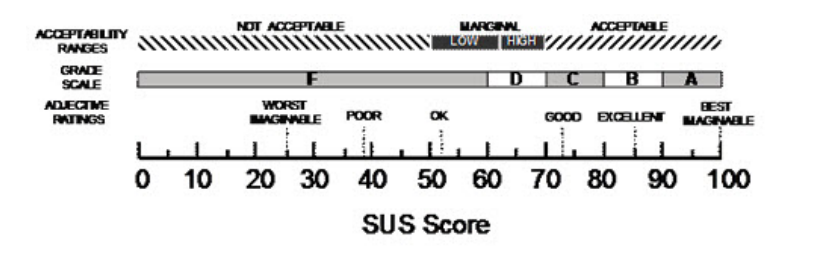
\includegraphics{pics/susscore}
		\caption{Nilai hasil evaluasi SUS}
		\centering
	\end{figure}
%-----------------------------------------------------------------------------%
\chapter{\babTiga}
\newcounter{babTigaNum}
\newcounter{defBabTiga}
\newcounter{contohBabTiga}

\addtocounter{babTigaNum}{3}

\label{bab3}

Pada \textit{abduction}, sering kali ditemukan bahwa \textit{abductive solution} yang didapatkan pada suatu proses \textit{abduction} ternyata memiliki relevansi dengan proses \textit{abduction} lainnya, mengindikasikan bahwa sebenarnya \textit{abductive solution} tersebut dapat dipergunakan kembali. Seperti yang sudah dijelaskan pada bagian sebelumnya, teknik \textit{tabling}, terlepas dari \textit{abduction}, dapat dipergunakan untuk mempergunakan kembali solusi yang sudah didapatkan \citep{swift1999tabling}. Secara konsep, \textit{tabling} tampaknya juga dapat diterapkan pada \textit{abduction}, yaitu untuk mempergunakan kembali \textit{abductive solution} yang sudah didapat. Namun praktisnya, \textit{abductive solution} dari \textit{goal G} tidak serta-merta dapat di-\textit{tabling} karena solusi tersebut secara khusus terkait dengan konteks pada proses \textit{abduction} jika diberikan \textit{goal G}. \textit{Abductive context} dari \textit{goal G} dapat diartikan sebagai himpunan \textit{abducible} yang memberikan informasi mengenai konteks dari proses \textit{abduction} yang digunakan untuk mencari \textit{abductive solution} dari \textit{goal G}.

Pada bagian ini, penulis akan menjelaskan teknik untuk mempergunakan kembali \textit{abductive solution} yang didapat dari suatu \textit{abductive context} pada \textit{abductive context} lainnya dengan memanfaatkan \textit{tabling}. Teknik melakukan \textit{tabling abductive solution} pada \textit{contextual abduction} ini disebut sebagai \textsc{Tabdual} \citep{saptawijaya2015tabdual}. Teknik ini didasari oleh \textsc{Abdual} \citep{alferes2004abduction}, yaitu suatu pendekatan yang dapat digunakan untuk melakukan komputasi terhadap \textit{abduction} pada Well-Founded Semantic. \textsc{Tabdual} merealisasikan teori transformasi program yang diberikan pada \textsc{Abdual} yaitu \textit{dual program transformation}, ditambah dengan adanya  \textit{tabling} untuk menyimpan \textit{abductive solution}, sekaligus mengatasi permasalahan yang ditemukan ketika melakukan \textit{abduction} pada \textit{goal} negatif. 

Penulis akan memulai menjelaskan dengan memberikan motivasi dan ide dasar diperlukannya \textit{tabling} dan \textit{abduction}, kemudian menunjukkan bagaimana konsep dan realisasi \textit{tabling} dan \textit{abduction} pada transformasi program yang dilakukan \textsc{Tabdual}.

\section{Motivasi dan Ide}

\textit{Contoh \thebabTigaNum.\stepcounter{contohBabTiga}\thecontohBabTiga}. Misal terdapat sebuah \textit{abductive framework} $\langle P_1, \{a/0,b/0 \},\emptyset \rangle$ dengan program $P_1$ sebagai berikut:
\begin{flalign*}
	& q \leftarrow a. \\
	& s \leftarrow q,b. \\
	& t \leftarrow s,q.
\end{flalign*}
Misal akan diberikan tiga buah \textit{query} untuk memberikan penjelasan dari \textit{q}, \textit{s}, dan \textit{t} secara berturut-turut.

\begin{itemize}
	\item \textit{Query} yang pertama, \textit{q}, terpenuhi hanya dengan memberikan $[a]$ sebagai \textit{abductive solution} untuk \textit{q} lalu menyimpannya ke \textit{table}.
	\item \textit{Query} berikutnya, \textit{s}, harus memenuhi dua \textit{subgoal} pada \textit{body}-nya, yaitu dengan mengeksekusi \textit{q} dan \textit{b}. Karena \textit{q} sudah pernah dieksekusi, solusi yang dihasilkan pada eksekusi \textit{q} sebelumnya dapat digunakan kembali, menghasilkan \textit{abductive context} $[a]$. Selanjutnya, $[a]$ yang dihasilkan dari \textit{subgoal q} ditambahkan dengan \textit{subgoal} berikutnya yaitu $[b]$ yang merupakan \textit{abducible}, menghasilkan \textit{abductive solution} $[a,b]$.
	\item Tidak jauh berbeda dengan \textit{query} sebelumnya, \textit{query t} akan mengekesekusi \textit{s} dan \textit{q}. Eksekusi dari \textit{subgoal s} menghasilkan \textit{abductive solution} yang sudah disimpan pada \textit{table} yaitu  $[a,b]$, sementara eksekusi dari \textit{q} mengahasilkan \textit{abductive solution} $[a]$ yang juga sudah disimpan pada \textit{table}. Karena $[a] \subseteq [a,b]$, maka \textit{query t} cukup  memberikan jawaban $[a,b]$ sebagai \textit{abductive solution}-nya.
\end{itemize}
Ilustrasi di atas menunjukkan bahwa $[a]$ sebagai \textit{abductive solution} yang didapatkan dari \textit{query} yang pertama \textit{q} dapat digunakan pada \textit{abductive context} dari dua \textit{query} lainnya berikutnya (dicontohkan dengan $[b]$ pada \textit{query s} dan $[a,b]$ pada \textit{query t}). Dapat dibayangkan jika \textit{q} memiliki \textit{subgoal} dengan jumlah yang sangat besar, tanpa \textit{tabling}, \textit{cost} yang diperlukan baik dari segi ruang dan waktu akan menjadi sangat mahal.

\label{fase}
\textsc{Tabdual} terdiri dari dua fase. Fase pertama yaitu \textit{program tansformation}, menghasilkan program \textit{output} yang dapat digunakan pada fase berikutnya, yaitu \textit{abduction} itu sendiri yang dapat dilakukan dengan memberikan \textit{query}.

\section{Transformasi Program}
Pada Contoh \thebabTigaNum.1 telah ditunjukkan dua unsur utama pada transformasi \textsc{Tabdual}:

\begin{itemize}
	\item \textit{Abductive context}, membawa informasi mengenai \textit{abductive solution} dari satu \textit{subgoal} ke \textit{subgoal} berikutnya pada \textit{body} dari sebuah \textit{rule}, juga dari \textit{head} dari sebuah \textit{rule} ke \textit{body}-nya, melalui \textit{input context} dan \textit{output context}.
	\item \textit{Tabled predicate}, menyimpan \textit{abductive solution} dari predikat yang muncul sebagai sebuah \textit{head} pada program untuk disimpan pada \textit{table}, sehingga \textit{abductive solution} yang sudah disimpan dapat dipergunakan kembali pada \textit{abductive context} yang berbeda.
\end{itemize}

Transformasi program pada \textsc{Tabdual} terdiri dari beberapa bagian, yaitu transformasi untuk melakukan \textit{tabling} terhadap \textit{abductive solution} (bagian 3.2.1), untuk melakukan \textit{abduction} pada \textit{goal} negatif (bagian 3.2.2), untuk menambahkan \textit{abducible} pada suatu \textit{abductive context} (bagian 3.2.3), dan untuk melakukan transformasi pada \textit{query} (bagian 3.2.4).

\subsection{\textit{Tabling Abductive Solution}}

Untuk merealisasikan ide yang ditunjukkan pada Contoh 3.1, \textsc{Tabdual} melakukan transformasi terhadap setiap \textit{rule} yang terdapat pada program menjadi dua buah \textit{rule}. \textit{Rule} pertama mendefinisikan \textit{tabled predikat} yang digunakan untuk memperoleh \textit{abductive solution}, dengan membawa \textit{abducible} pada \textit{rule} tersebut sebagai \textit{input context} untuk melakukan \textit{abduction} mulai dari \textit{subgoal} pertama, satu per satu hingga ke \textit{subgoal} terakhir, lalu menyimpan \textit{abductive solution} yang didapat ke dalam \textit{table}. Sementara itu, \textit{rule} kedua hasil transformasi digunakan untuk mendapatkan \textit{abductive solution} yang sudah disimpan pada \textit{table} sehingga dapat dipergunakan kembali pada \textit{abductive context} yang berbeda.

Transformasi untuk membentuk kedua \textit{rule} di atas didefinisikan secara formal sebagai pada Definisi \thebabTigaNum.1.
\\

Untuk selanjutnya, $\bar{t}$ digunakan untuk menyatakan $[t_1, \textellipsis ,t_n]$, $n \geq 0$. Untuk sebuah predikat $p/n$, $p(\bar{t})$ digunakan untuk menyatakan $p(t_1, \textellipsis , t_n)$. Secara khusus, $\bar{X}$ digunakan untuk menyatakan $[X_1, \textellipsis , X_n]$, $p(\bar{X})$ untuk menyatakan $p(X_1, \textellipsis , X_n)$, dan $p(\bar{X},Y,Z)$ untuk menyatakan $p(X_1, \textellipsis , X_n,Y,Z)$, dengan seluruh variabel yang disebutkan merupakan variabel yang berbeda-beda.
\\

\noindent \textbf{Definisi \thebabTigaNum.\stepcounter{defBabTiga}\thedefBabTiga: Transformasi untuk \textit{tabling abductive solution}.} Diberikan sebuah \textit{abductive framework} $\langle  P,\mathcal{AB},\mathcal{IC} \rangle$. $H_r$ dan $\mathcal{B}_r$ berturut-turut menunjukkan \textit{head} dan \textit{body} dari sebuah \textit{rule} $r \in P$. Himpunan $\mathcal{A}_r \subseteq \mathcal{B}_r$ menunjukkan himpunan \textit{abducible} (positif ataupun negatif) pada $r \in P$, dan $r'$ menunjukkan \textit{rule} sedemikian sehingga $H_{r'} = H_r$ dan $\mathcal{B}_{r'} = \mathcal{B}_r \backslash \mathcal{A}_r$.

\begin{enumerate}
	\item Untuk setiap $rule \ r \in P$ dengan $r'$ yaitu $l(\hat{t}) \leftarrow L_1, \textellipsis , L_M$, didefinisikan $\tau'(r)$:
	\begin{displaymath}
		l_{ab}(\bar{t},E_m) \leftarrow \alpha(L_1), \textellipsis , \alpha(L_m).
	\end{displaymath}
	dengan $\alpha$ didefinisikan sebagai:
	\begin{displaymath}
	\alpha(L_i) = 
	\begin{cases}
	l_i(\bar{t}_i,E_{i-1},E_i) & \text{untuk $L_i = l_i(\bar{t}_i)$} \\
	not\_l_i(\bar{t}_i,E_{i-1},E_i) & \text{untuk $L_i = not \ l_i(\bar{t}_i)$}
	\end{cases}
	\end{displaymath}
	dengan $1 \leq i \leq m$, $E_1$ adalah variabel baru, dan $E_0 = \mathcal{A}_r$. Dapat dilihat bahwa $E_i$ disediakan \textit{abductive context}.
	
	\item Untuk setiap predikat $p/n$ yang menjadi \textit{head} dari sebuah \textit{rule} pada \textit{P}, didefinisikan $\tau^+(p)$:
	\begin{displaymath}
		p(\bar{X},I,O) \leftarrow p_{ab}(\bar{X},E), produce\_context(O,I,E).
	\end{displaymath}
	dengan $produce\_context(O,I,E)$ adalah predikat sistem \textsc{Tabdual} yang digunakan untuk membentuk \textit{O} dengan menambahkan setiap $e \in E$ pada $I$, sekaligus melakukan pengecekan apakah \textit{I} konsisten dengan \textit{E}, yaitu apakah terdapat dua literal yang saling berlawanan pada \textit{I} dan \textit{E}.
\end{enumerate}

\subsection{\textit{Abduction} pada \textit{Goal} Negatif}

Untuk melakukan \textit{abduction} pada \textit{goal} negatif, transformasi pada \textsc{Tabdual} menerapkan \textit{dual program transformation} pada \textsc{Abdual} \citep{alferes2004abduction}. Tujuan utama dari menggunakan \textit{dual program transformation} yaitu untuk dapat memperoleh solusi dari \textit{goal} negatif \textit{not G} tanpa harus menegasikan seluruh \textit{abductive solution} dari \textit{G}.

Ide dari \textit{dual program transformation} yaitu mendefinisikan, untuk setiap atom \textit{A} dan himpunan \textit{rule} mengenai \textit{A} $\mathcal{R}_A$ pada program \textit{P}, himpunan \textit{dual rule} yang \textit{head}-nya adalah \textit{not\_A}, sedemikian sehingga \textit{not\_A} bernilai \textit{true} jika dan hanya jika \textit{A} bernilai \textit{false} sesuai dengan $\mathcal{R}_A$ menurut semantik yang digunakan oleh program \textit{P}. Alih-alih menggunakan \textit{goal} negatif \textit{not A}, \textit{dual program transformation} menggunakan atom \textit{not\_A} yang bersesuaian. 

\textit{Dual program transformation} membentuk dua buah jenis \textit{rule} (\textit{atau layer}) yang berbeda. \textit{First layer} dari \textit{dual program transformation}, atau \textit{first layer dual rule}, dari sebuah predikat \textit{p} pada program \textit{P} merupakan \textit{rule} $not\_p$ yang didefinisikan untuk mem-\textit{falsify} negasi dari \textit{p}, yaitu $not \ p$, sekaligus dengan membawa \textit{input context} yang diberikan untuk melakukan \textit{abduction} pada setiap \textit{subgoal-subgoal}-nya sehingga menghasilkan \textit{abductive solution} dari \textit{p}. \textit{Subgoal-subgoal} dari \textit{first layer dual rule} itu sendiri merupakan \textit{second layer dual rule} $p^{*i}$ yang didefinisikan berdasarkan \textit{rule-rule} mengenai \textit{p} yang terdapat pada program, digunakan untuk mem-\textit{falsify} tiap \textit{rule} pada \textit{body} dari \textit{rule} mengenai \textit{p}, tentunya setelah dinegasikan.

Tranformasi yang membentuk kedua \textit{layer} dari \textit{dual rule} didefinisikan secara formal pada Definisi \thebabTigaNum.2.
\\

\noindent \textbf{Definisi \thebabTigaNum.\stepcounter{defBabTiga}\thedefBabTiga: Transformasi untuk membentuk \textit{dual rule}.} Diberikan sebuah \textit{abductive framework} $\langle  P,\mathcal{AB},\mathcal{IC} \rangle$. Misal $P^+ = P \cup \mathcal{IC}$.

\begin{enumerate}
	\item Untuk setiap predikat $p/n$ yang memiliki \textit{rule} pada $P^+$ seperti berikut:
	\begin{flalign*}
		p(\bar{t}_1) 	& \leftarrow L_{11}, \textellipsis , L_{1n_1}. \\
						& \vdots \\
		p(\bar{t}_m) 	& \leftarrow L_{m1}, \textellipsis , L_{mn_m}. \\
	\end{flalign*}
	dengan $n_i \geq 0, 1 \leq i \leq m$:
	\begin{enumerate}
		\item \textit{First layer dual rule} didefinisikan sebagai $\tau^-(p)$:
		\begin{displaymath}
			not\_p(\bar{X},T_0,T_m) \leftarrow p^{*1}(\bar{X},T_0,T_1), \textellipsis , p^{*1}(\bar{X},T_{m-1},T_m).
		\end{displaymath}
		dengan $T_i, i \leq i \leq m$ adalah variabel baru yang disediakan sebagai \textit{abductive context}.
		\item \textit{Second layer dual rule} didefinisikan sebagai $\tau^*(p) = \bigcup\limits_{i=1}^{m} \tau^{*i}(p)$, dengan $\tau^{*i}(p)$ merupakan himpunan terkecil yang mengandung \textit{rule-rule} sebagai berikut:
		\begin{flalign*}
			p^{*i}(\bar{X},I,I)	& \leftarrow \bar{X} \neq \bar{t}_i. \\
			p^{*i}(\bar{X},I,O) & \leftarrow \sigma(L_{i1},I,O). \\
			& \vdots \\
			p^{*i}(\bar{X},I,O) & \leftarrow \sigma(L_{in_i},I,O).
		\end{flalign*}
		dengan $\sigma$ didefinisikan sebagai berikut:
		\begin{displaymath}
		\sigma(L_{ij},I,O) = 
		\begin{cases}
		l_{ij}(\bar{t}_{ij},I,O) 	& \text{jika $L_i$ adalah \textit{default} literal $not \ l_{ij}(\bar{t}_{ij})$} \\
									& \text{atau \textit{abducible} negatif $l_{ij}^*(\bar{t}_{ij})$} \\
		not\_l_{ij}(\bar{t}_{ij},I,O) & \text{jika $L_i$ adalah atom $l_{ij}(\bar{t}_{ij})$} \\
		l_{ij}^*(\bar{t}_{ij},I,O)	& \text{jika $L_i$ adalah \textit{abducible} positif $l_{ij}(\bar{t}_{ij})$}
		\end{cases}
		\end{displaymath}
		Untuk kasus $p/0$, \textit{rule} $p^{*i}(\bar{X},I,I) \leftarrow \bar{X} \neq \bar{t}_i$ dihilangkan karena $\bar{X}$ dan $\bar{t}_i$ merupakan $[]$.
	\end{enumerate}
	
	\item Untuk setiap predikat $r/n$ pada $P^+ (n \geq 0)$ yang tidak memiliki \textit{rule}, didefinisikan $\tau^-(r)$:
	\begin{displaymath}
		not\_r(\bar{X},I,I).
	\end{displaymath}
	Secara khusus, jika $\mathcal{IC} = \emptyset$, didefinisikan $\tau^-(r): not\_\bot(I,I)$. 
\end{enumerate}

\subsection{\textit{Transformasi \textit{Abducible}}}

\textit{Abduction} pada \textsc{Tabdual} dilakukan dengan melakukan transformasi pada setiap \textit{abducible} menjadi \textit{rule} yang dapat menambahkan \textit{abducible} pada \textit{abductive context} yang sudah ada. Spesifikasi untuk melakukan transformasi terhadap \textit{abducible} akan diberikan secara formal pada Definisi \thebabTigaNum.3.
\\

\noindent \textbf{Definisi \thebabTigaNum.\stepcounter{defBabTiga}\thedefBabTiga: Transformasi\ \textit{abducible}.} Diberikan sebuah \textit{abductive framework} $\langle  P,\mathcal{AB},\mathcal{IC} \rangle$. Untuk setiap $a/n \in \mathcal{AB}$, didefinisikan $\tau^\circ(a)$ yaitu himpunan terkecil yang mengandung \textit{rule}:
\begin{flalign*}
	a(X_1, \textellipsis , X_n,I,O) & \leftarrow insert\_abducible(a(X_1, \textellipsis , X_n),I,O). \\
	a^*(X_1, \textellipsis , X_n,I,O) & \leftarrow insert\_abducible(a^*(X_1, \textellipsis , X_n),I,O).
\end{flalign*}
dengan $insert\_abducible(A,I,O)$ merupakan predikat sistem \textsc{Tabdual} yang menambahkan \textit{abducible A} ke \textit{input context I} dan menghasilkan \textit{output context O}. Predikat ini juga mempertahankan konsistensi dari \textit{abductive context I} jika ditambahkan oleh \textit{abducible A}.
\\

Spesifikasi program transformation \textsc{Tabdual} secara utuh akan diberikan pada Definisi \thebabTigaNum.4.
\\

\noindent \textbf{Definisi \thebabTigaNum.\stepcounter{defBabTiga}\thedefBabTiga: Transformasi\ \textsc{Tabdual}.} Diberikan \textit{abductive framework} $\mathcal{F} = \langle  P,\mathcal{AB},\mathcal{IC} \rangle$, $\mathcal{P}$ adalah himpunan predikat yang terdapat pada \textit{P}, dan $P^+ = P \cup \mathcal{IC}$. Menggunakan definisi-definisi transformasi sebelumnya didapatkan:

\begin{itemize}
	\item $\tau'(\mathcal{F}) = \{\tau'(r) \ | \ r \in P  \}$
	\item $\tau^+(\mathcal{F}) = \{\tau^+(p) \ | \ p \in \mathcal{P} \ \text{yang memiliki \textit{rule} pada} \ P \}$
	\item $\tau^-(\mathcal{F}) = \{\tau^-(p) \ | \ p \in \mathcal{P} \cup \{ \bot\} \}$
	\item $\tau^*(\mathcal{F}) = \{\tau^*(p) \ | \ p \in \mathcal{P} \cup \{ \bot\} \ \text{yang memiliki \textit{rule} pada} \ P \}$
	\item $\tau^\circ(\mathcal{F}) = \{\tau^\circ(a) \ | \ a \in \mathcal{AB} \}$
\end{itemize}

maka transformasi \textsc{Tabdual} didefinisikan sebagai:
\begin{displaymath}
	\tau(\mathcal{F}) = \tau'(\mathcal{F}) \cup \tau^+(\mathcal{F}) \cup \tau^-(\mathcal{F}) \cup \tau^*(\mathcal{F}) \cup \tau^\circ(\mathcal{F})
\end{displaymath}

\subsection{\textit{Transformasi \textit{Query}}}
\label{transquery}

Sebagai konsekuensi dari transformasi \textsc{Tabdual}, \textit{query} terhadap program juga harus di-\textit{transform}:

\begin{itemize}
	\item \textit{Goal} positif $G$ cukup di-\textit{transform} dengan menambahkan dua buah argumen untuk menyatakan \textit{input context} dan \textit{putput context}.
	\item \textit{Goal} negatif $not \ G$ di-\textit{transform} dengan mengubah namanya menjadi $not\_G$ serta ditambahkan dua buah argumen untuk menyatakan \textit{input context} dan \textit{putput context}.
\end{itemize}

Selanjutnya, \textit{query} yang diberikan juga harus memenuhi seluruh \textit{integrity constraint} yang ada. Hal ini dapat dilakukan dengan menambahkan \textit{goal} $not\_\bot/2$ yang menyatakan \textit{dual rule} dari \textit{integrity constraint}. Definisi \thebabTigaNum.5 memberikan definisi formal untuk melakukan transformasi pada \textit{query}.
\\

\noindent \textbf{Definisi \thebabTigaNum.\stepcounter{defBabTiga}\thedefBabTiga: Transformasi\ \textit{query}.} Diberikan \textit{abductive framework} $\mathcal{F} = \langle  P,\mathcal{AB},\mathcal{IC} \rangle$ dan query \textit{Q}:
\begin{displaymath}
	\text{\texttt{?}}- \ G_1, \textellipsis , G_m.
\end{displaymath}
\textsc{Tabdual} melakukan transformasi $query \ Q$ menjadi $\Delta(Q)$:
\begin{displaymath}
	\text{\texttt{?}}- \ \delta(G_1), \textellipsis , \delta(G_m), not\_\bot(T_m,O).
\end{displaymath}
dengan $\delta$ didefinisikan sebagai:
\begin{displaymath}
\alpha(L_i) = 
\begin{cases}
g_i(\bar{t}_i,T_{i-1},T_i) 		& \text{jika $G_i = g_i(\bar{t}_i)$} \\
not\_g_i(\bar{t}_i,E_{i-1},T_i) 	& \text{jika $G_i = not \ g_i(\bar{t}_i)$}
\end{cases}
\end{displaymath}

\section{Aspek Implementasi}

\textsc{Tabdual} diimplementasikan menggunakan XSB Prolog \citep{swift2012xsb}, sehingga dapat memanfaatkan fitur-fitur yang sudah ada. Namun di sisi lain, sebagai konsekuensinya implementasi yang dibuat juga harus disesuaikan dengan \textit{behavior} yang dimiliki XSB Prolog.

\subsection{\textit{Grounding Dualized Negated Subgoals}}

\textit{Contoh \thebabTigaNum.\stepcounter{contohBabTiga}\thecontohBabTiga}. Misal terdapat \textit{abductive framework} $\langle  P_4,\{a/1 \},\mathcal{IC}_4 \rangle$ dengan program $P_4$ sebagai berikut:
\begin{flalign*}
	q(1) & .  \\
	r(X) &\leftarrow a(X).
\end{flalign*}
dan $\mathcal{IC}_4$:
\begin{flalign*}
	\bot & \leftarrow q(X),r(X).
\end{flalign*}
Transformasi \textsc{Tabdual} akan menghasilkan program:
\begin{flalign*}
&&&&&& 1. \ & q_{ab}(1,[ \ ]). & & \\
&&&&&& 2. \ & q(X,I,O) & \leftarrow & \ q_{ab}(X,E),produce\_context(O,I,E). &&&&&& \\
&&&&&& 3. \ & not\_q(X,I,O) & \leftarrow & \ q^{*1}(X,I,O). &&&&&& \\
&&&&&& 4. \ & q^{*1}(X,I,I) &  \leftarrow & \ X \ \backslash = 1. &&&&&& \\
\\
&&&&&& 5. \ & r_{ab}(X,[a(X)]). & & \\
&&&&&& 6. \ & r(X,I,O) & \leftarrow & \ r_{ab}(X,E),produce\_context(O,I,E). &&&&&& \\
&&&&&& 7. \ & not\_r(X,I,O) & \leftarrow & \ r^{*1}(X,I,O). &&&&&& \\
&&&&&& 8. \ & r^{*1}(X,I,O) & \leftarrow & \ X \ \backslash = \_. &&&&&& \\
&&&&&& 9. \ & r^{*1}(X,I,O) & \leftarrow & \ a^{*}(X,I,O). &&&&&& \\
\\
&&&&&& 10. \ & not\_\bot(I,O) & \leftarrow & \ \bot^{*1}(I,O). &&&&&& \\
&&&&&& 11. \ & \bot^{*1}(I,O) & \leftarrow & \ not\_q(X,I,O). &&&&&& \\
&&&&&& 12. \ & \bot^{*1}(I,O) & \leftarrow & \ not\_r(X,I,O). &&&&&& 
\end{flalign*}
Lalu diberikan \textit{query} $q(1)$, yang di-\textit{transform} menjadi:
\begin{displaymath}
	\text{\texttt{?}}- q(1,[ \ ],T),not\_\bot(T,O).
\end{displaymath}
progam akan memberikan \textit{abductive solution} $[a^*(X)]$ (tidak \textit{ground}), tidak sesuai dengan \textit{abductive solution} yang seharusnya diberikan yaitu $[a^*(1)]$. Kesalahan ini disebabkan karena ketika program mencari solusi, \textit{fail}-nya \textit{subgoal} dari \textit{rule} 11 $not\_q(X,I,O)$ menyebabkan program mengekesekusi $not\_r(X,I,O)$ pada \textit{rule} 12 sebagai alternatif lain dari \textit{goal} $\bot^{*1}(I,O)$, namun dengan $X$ yang tidak \textit{ground} karena memang belum diinstansiasi.

Untuk memperbaiki kesalahan ini, \textit{dualized negated subgoal} (pada contoh di atas yaitu \textit{subgoal} dari \textit{rule} 4, 8, 9, 11, 12) perlu untuk di-\textit{ground}-kan terlebih dahulu. \textit{Grounding subgoal} ini dapat dilakukan dengan tetap mengikutsertakan pada \textit{second layer dual rule} literal-literal positif yang pada \textit{rule} aslinya terdapat sebelum predikat yang sedang di-\textit{dual}-kan. Dengan begitu, \textit{rule} 12 pada program di atas akan menjadi:
\begin{displaymath}
	\bot^{*1}(I,O) \leftarrow q(X,I,T),not\_r(X,T,O).
\end{displaymath}
Adanya $q(X,I,T)$ sebagai \textit{subgoal} sebelum $not\_r(X,T,O)$ pada \textit{rule} 12 menyebabkan $X$ akan diinstansiasi terlebih dahulu menggunakan \textit{rule} 4 sehingga \textit{query} $q(1)$ menghasilkan \textit{abductive solution} yang sesuai yaitu $[a^*(1)]$

\subsection{\textit{Non-Ground Negative Goal}}

\textit{Contoh \thebabTigaNum.\stepcounter{contohBabTiga}\thecontohBabTiga}. Misal terdapat \textit{abductive framework} $\langle  P_5,\{a/1 \},\emptyset \rangle$ dengan program $P_5$ sebagai berikut:
\begin{flalign*}
	p(1) & \leftarrow a(1) .  \\
	p(2) & \leftarrow a(2) .  
\end{flalign*}

\textit{Query} $p(X)$ pada program diatas akan memberikan \textit{abductive solution} yang sesuai yaitu $[a(1)]$ untuk $X = 1$ dan $[a(2)]$ untuk $X = 2$. Sementara itu, \textit{query} $not \ p(X)$ memberikan hasil yang tidak sesuai. \textit{Abuctive solution} seharusnya yang dihasilkan yaitu $[a^*(1),a^*(2)]$ untuk apa pun instansiasi $X$, namun \textsc{Tabdual} memberikan \textit{abductive solution} $[a*(1)]$ untuk $X = 1$. 

Berikut ini merupakan definisi predikat $not\_p/3$:
\begin{flalign*}
	&&&&&& 1. \ & not\_p(X,I,O) & \leftarrow & \ p^{*1}(X,I,T), p^{*2}(X,T,O). &&&&&& \\
	&&&&&& 2. \ & p^{*1}(X,I,O) & \leftarrow & \ X \ \backslash = 1. &&&&&& \\
	&&&&&& 3. \ & p^{*1}(X,I,O) & \leftarrow & \ a^*(1,I,O). &&&&&& \\
	&&&&&& 4. \ & p^{*2}(X,I,O) & \leftarrow & \ X \ \backslash = 2. &&&&&& \\
	&&&&&& 5. \ & p^{*2}(X,I,O) & \leftarrow & \ a^*(2,I,O). &&&&&&
\end{flalign*}
dan query $not \ p(X)$ yang dihasilkan oleh transformasi \textsc{Tabdual}:
\begin{displaymath}
\text{\texttt{?}}- not\_p(X,[ \ ],N),not\_\bot(N,O).
\end{displaymath}
Goal $not\_p(X,[ \ ],N)$ pertama-tama mengeksekusi $p^{*1}(X,I,O)$ dengan $I = [ \ ]$, lalu dengan menggunakan \textit{rule} 3 berhasil memberikan $T = [a^*(1)]$ dengan $X$ diinstansiasi dengan 1. Selanjutnya, \textit{subgoal} kedua yaitu $p^{*2}(X,I,O)$, dieksekusi dengan instansiasi $X$ dan $T$ yang sama ($X = 1$ dan $T = [a^*(1)]$), dan dengan menggunakan \textit{rule} 4, $p^{*2}(X,I,O)$ berhasil memberikan $O = [a^*(1)]$, tetap dengan $X$ yang diinstansiasi dengan 1. $[a^*(1)]$ yang merupakan \textit{abductive solution} dari \textit{goal} pertama pada \textit{query} dibawa sebagai $N$ ke \textit{goal} berikutnya yaitu $not\_\bot(N,O)$. Dikarenakan tidak terdapat \textit{integrity constraint}, \textit{subgoal} $not\_\bot(N,O)$ menghasilkan $O$ yang sama dengan $N$, menghasilkan $[a^*(1)]$ sebagai \textit{abductve solution} dari \textit{query} $not \ p(X)$.

Dapat dilihat bahwa ketidaksesuaian \textit{abductive solution} yang dihasilkan terjadi karena terdapat \textit{shared variable} pada kedua \textit{subgoal} dari $not\_p(X,I,O)$, yaitu $X$, menyebabkan $p^{*1}(X,I,O)$ dan $p^{*2}(X,I,O)$ dieksekusi dengan $X$ yang sama. Seharusnya, kedua \textit{subgoal} ini dieksekusi dengan $X$ yang saling independen satu sama lain. Ketidaksesuaian ini dapat diatasi dengan mengubah definisi dari predikat $not\_p/3$ menjadi:
\begin{flalign*}
	not\_p(X,I,O) \leftarrow & \ copy\_term([X],[X_1]),p^{*1}(X_1,I,T), \\
	& copy\_term([X],[X_2]) p^{*2}(X_2,T,O).
\end{flalign*}
dengan predikat \textit{copy\_term$/$}2 merupakan predikat \textit{built-in} yang disediakan oleh Prolog. \textit{copy\_term$/$}2 ditambahkan sebelum masing-masing \textit{subgoal} dari \textit{first layer dual rule} (dalam kasus ini sebelum $p^{*1}(X,I,O)$ dan $p^{*2}(X,I,O)$), digunakan untuk memberikan \textit{varian} baru terhadap $X$ agar dapat digunakan secara independen.
\subsection{Transformasi Fakta}
\label{transfact}

\textsc{Tabdual} melakukan transformasi pada seluruh predikat yang ada pada program, termasuk predikat yang sebenarnya hanya berupa fakta yang bahkan tidak menginduksikan \textit{abduction} sama sekali. Oleh karena itu, transformasi yang lebih sederhana dapat diterapkan pada predikat-predikat yang hanya berupa fakta.

Misalkan terdapat predikat $q/1$ yang hanya berupa fakta seperti berikut:
\begin{flalign*}
	q(1). \quad \quad q(2). \quad \quad q(3).
\end{flalign*}
\textit{Rule} transformasi untuk $q/1$ yang telah didefinisikan pada Definisi 3.1, yaitu $q_{ab}/1$ dan $q/3$ dapat digantikan dengan satu buah \textit{rule} positif berikut:
\begin{flalign*}
	q(X,I,I) \leftarrow q(X).
\end{flalign*}
dan \textit{dual rule} untuk $q/1$ yang telah didefinisikan pada Definisi 3.2 juga cukup digantikan dengan satu buah \textit{rule} negatif berikut:
\begin{flalign*}
	not\_q(X,I,I) \leftarrow not \ q(X).
\end{flalign*}

Transformasi untuk fakta seperti predikat $q/1$ bersifat independen terhadap jumlah fakta yang ada, sehingga dapat dipisahkan dari keseluruhan program dan dikelompokkan menjadi bagian yang bersifat \textit{non-abductive} untuk diproses secara khusus. Pada \textsc{Tabdual}, bagian program yang bersifat \textit{non-abductive} dapat dipisahkan dengan \textit{indentifier} \textit{beginProlog} dan \textit{endProlog}. Program yang terdapat diantara kedua identifier ini tidak akan di-\textit{transform} oleh \textsc{Tabdual}, melainkan hanya akan dibaca dan ditulis ulang ke program \textit{output}.

\subsection{\textit{Dual Transformation by Need}}
\label{dualbyneed}

Transformasi yang dilakukan oleh \textsc{Tabdual} bersifat \textit{once for all}, yaitu men-\textit{transform} seluruh predikat, atom, dan \textit{abducible} yang terdapat pada program, tanpa pertimbangan apakah predikat/atom/\textit{abducible} yang di-\textit{transform} akan digunakan pada fase \textit{abduction} atau tidak. Praktis, transformasi seperti ini harus dihindari dikarenakan \textit{cost} yang diperlukan terlalu besar untuk melakukan transformasi yang belum tentu digunakan. Salah satu solusi untuk mengatasi permasalahan ini yaitu dengan melakukan transformasi \textit{dual rule} secara \textit{by need}, yaitu dengan tidak membentuk \textit{dual rule} pada fase transformasi, melainkan pada saat fase \textit{abduction} ketika \textit{dual rule} tersebut dibutuhkan untuk dieksekusi. Program \textit{output} yang dihasilkan tetap mengandung \textit{first layer dual rule}, namun tidak \textit{second layer dual rule} yang jumlahnya relatif lebih banyak. \textit{Second layer dual rule} akan dibentuk \textit{on-the-fly} pada fase \textit{abduction} dengan bantuan predikat sistem \textsc{Tabdual} yang dikhususkan untuk membentuk definisi konkrit dari \textit{second layer dual rule} ini.
\\

\noindent \textit{Contoh \thebabTigaNum.\stepcounter{contohBabTiga}\thecontohBabTiga}. Lihat kembali Contoh 3.2. Transformasi \textit{dual by need} menghasilkan \textit{first layer dual rule} yang sama yaitu $not\_p(X,I,O) \leftarrow p^{*1}(X,I,T), p^{*2}(X,T,O)$, sementara \textit{second layer dual rule} yang dihasilkan menjadi, untuk setiap $i \in \{1,2\}$:
\begin{flalign*}
	p^{*i}(X,I,O) \leftarrow dual(i,p,I,O).
\end{flalign*}
dengan predikat $dual/4$ merupakan predikat sistem \textsc{Tabdual} yang didefinisikan untuk memudahkan \textit{dual transformation by need}. Eksekusi $dual(i,p,I,O)$ di atas akan membentuk \textit{dual rule} yang bersifat \textit{generic}, yaitu \textit{dual rule} yang belum diberikan \textit{context} berdasarkan \textit{rule} ke-$i$ dari $p/0$. Setelah \textit{dual rule} dibentuk pada fase \textit{abduction}, $dual/4$ akan melakukan instansiasi dengan \textit{input context} diberikan kemudian melakukan eksekusi terhadap \textit{dual rule} yang telah diinstansiasi.

Meskipun \textit{dual transformation by need} dapat mengurangi jumlah \textit{second layer dual rule} pada program \textit{output}, melakukan transformasi \textit{on-the-fly} menyebabkan dibutuhkannya \textit{cost} tambahan pada fase \textit{abduction}. \textit{Cost} tambahan ini dapat dikurangi dengan menyimpan \textit{dual rule} yang sudah pernah dibentuk agar dapat dipergunakan kembali. 

Menariknya, XSB Prolog menyediakan mekanisme untuk menyimpan dan memanipulasi fakta-fakta pada progam logika dengan menggunakan \textit{trie} \citep{swift2015xsb}. \textit{Trie} merupakan sebuah struktur data yang dapat digunakan untuk menyimpan data, misalnya \textit{string}, secara kompak dengan memanfaatkan representasi \textit{prefix-prefix} dari data yang disimpan. Kumpulan fakta berikut:
\begin{displaymath}
	\{rt(a,f(a,b),a), rt(a,f(a,X),Y), rt(b,V,d) \}
\end{displaymath}
disimpan pada \textit{trie} seperti pada gambar di bawah ini.
\begin{figure}
	\centering
	\includegraphics[scale=0.7]
	{trie.png}
	\caption{Fakta yang disimpan pada \textit{trie} \citep{swift2015xsb}.}
	\label{trie}
\end{figure}

\textit{Dual rule} yang dibentuk dapat direpresentasikan sebagai sebuah fakta, memungkinkan untuk disimpan di dalam sebuah \textit{trie} sehingga dapat dipergunakan kembali tanpa harus me-\textit{transform} ulang. XSB Prolog sudah menyediakan predikat untuk menyimpan term ke dalam \textit{trie}, melakukan unifikasi dengan sebuah term pada \textit{trie}, dan beberapa predikat lainnya yang dapat digunakan untuk memanipulasi isi serta bentuk dari \textit{trie}.
%-----------------------------------------------------------------------------%
\chapter{\babEmpat}
%-----------------------------------------------------------------------------%
Pada bab ini penulis akan menjelaskan implementasi \textsc{Tabdual} yang dibuat oleh penulis.

\section{Terminologi}

Pada bagian ini penulis menjelaskan beberapa ketentuan dan istilah yang digunakan pada bagian-bagian berikutnya, yaitu:

\begin{itemize}
	\item Pada Prolog, variabel diawali dengan huruf kapital sedangkan term dan predikat diawali dengan huruf non-kapital.
	\item \textit{Consult} berarti melakukan kompilasi program Prolog dan memuat hasil kompilasi program tersebut ke dalam \textit{database} XSB sehingga program tersebut menjadi \textit{knowledge base}.
	\item \textit{Database} berarti kumpulan predikat-predikat yang disimpan pada \textit{environment} XSB dan dijadikan sebagai \textit{knowledge base} selama eksekusi. Predikat-predikat yang ada pada \textit{database} dapat berasal dari program yang di-\textit{consult} (membentuk \textit{database} statis) ataupun ditambahkan selama eksekusi suatu program (membentuk \textit{database} dinamis). Selama eksekusi, predikat yang sudah ditambahkan ke dalam \textit{database} dinamis dapat dimanipulasi sesuai kebutuhan program.
	\item \textit{Dual transformation by need} mengacu pada proses transformasi dual \textit{by need} yang sudah dijelaskan pada bagian ???.
\end{itemize}

\section{Spesifikasi \textsc{Tabdual}}

\subsection{Tahapan \textsc{Tabdual}}

Seperti yang sudah dijelaskan pada \hyperref[fase]{\textcolor{blue}{bagian 3.1}}, secara garis besar, \textsc{Tabdual} terbagi menjadi 2 fase:

\begin{enumerate}
	\item \textbf{Transformasi}. Pada fase ini, \textsc{Tabdual} akan melakukan transformasi program \textit{input} \textit{P} menjadi program \textit{output} \textit{P$'$} yang dapat mengaplikasikan \textit{contextual abduction}. Transformasi dilakukan sesuai dengan aturan-aturan transformasi yang sudah dijelaskan pada \hyperref[bab2]{\textcolor{blue}{bagian 2}}.
	\item \textbf{Abduction}. \textit{Contextual abduction} dapat dilakukan setelah program \textit{input} \textit{P} berhasil di-\textit{transform} menjadi program \textit{output} \textit{P$'$}. Praktis, \textit{P$'$} harus di-\textit{consult} terlebih dahulu sebelum kita dapat memberikan \textit{query} dan melakukan \textit{contextual abduction}.
\end{enumerate}

Penjelasan lebih detil mengenai setiap fase akan penulis jabarkan pada bagian-bagian berikutnya.

\subsection{Berkas Implementasi \textsc{Tabdual}}
Agar dapat digunakan secara modular, implementasi \textsc{Tabdual} dipecah ke dalam empat buah berkas yang berbeda. Keeempat berkas tersebut yaitu:

\begin{itemize}
	\item \textit{tabdual.p}. Berkas ini berisi implementasi utama dari \textsc{Tabdual}, baik implementasi untuk fase transformasi maupun implementsai untuk fase \textit{abduction}. Berkas ini adalah berkas yang harus di-\textit{consult} untuk dapat menggunakan \textsc{Tabdual}. Berkas-berkas lain yang diperlukan selama menggunakan \textsc{Tabdual} akan di-\textit{consult} melalui berkas ini.
	\item \textit{system.p}. Berkas ini berisi predikat-predikat bantuan dan predikat-predikat yang didefinisikan secara khusus yang akan digunakan  oleh \textsc{Tabdual} ketika melakukan \textit{tabling}, \textit{contextual abduction}, dan \textit{answer subsumption}. 
	\item \textit{read\_clause.p} Berkas ini berisi predikat-predikat yang dikhususkan untuk membaca program \textit{input} agar dapat diproses dan ditransformasikan menggunakan \textsc{Tabdual}.
	\item \textit{write\_clause.p}. Berkas ini berisi predikat-predikat yang dikhususkan untuk menulis transformasi dari program \textit{input} yang dihasilkan menggunakan \textsc{Tabdual} ke program \textit{output}.
\end{itemize}

\subsection{Program \textit{Input} \textsc{Tabdual}}
Program \textit{input} yang ingin di-\textit{transform} menggunakan \textsc{Tabdual} harus memenuhi kriteria-kriteria berikut:

\begin{itemize}
	\item \textit{Rule} ditulis dalam bentuk \textit{H $\leftarrow B_1, \textellipsis,B_n.$}, dengan operator $\leftarrow$ ditulis sebagai "<-" (tanda lebih kecil dari dari lalu \textit{dash}).
	\item Fakta ditulis dalam bentuk \textit{H}. saja tanpa operator $\leftarrow$.
	\item \textit{Abducible} pada program ditulis sebagai fakta menggunakan predikat \textit{abds$/$}1. Argumen dari predikat ini yaitu himpunan \textit{abducible} yang ada pada program beserta dengan \textit{arity}-nya, direpresentasikan sebagai sebuah \textit{list}.
	\item Predikat-predikat yang hanya berupa fakta dan \textit{rule-rule} yang tidak ingin di-\textit{transform} ditulis terpisah di bagian paling atas program \textit{input}, di antara predikat \textit{beginProlog} dan \textit{endProlog}. 
	\item Setiap \textit{rule} dan fakta yang ditulis diakhiri dengan tanda titik (".").
\end{itemize}

\noindent Agar lebih jelas, berikut ini merupakan contoh program yang diterima sebagai program \textit{input} untuk \textsc{Tabdual}.
\\

\begin{lstlisting}[
caption=Contoh program \textit{input} yang diterima \textsc{Tabdual},
style=prolog,
numbers=left,
xleftmargin=3em
]
beginProlog.
q(1).
q(2).
endProlog.

abds([a/1,b/1]).

r(X) <- a(X).
s(X) <- b(X).

<- q(X), r(X), s(X).
\end{lstlisting}

\noindent Dan berikut ini merupakan contoh yang tidak diterima.
\\

\begin{lstlisting}[language=Prolog,
caption=Contoh program \textit{input} yang tidak diterima \textsc{Tabdual},
style=prolog,
numbers=left,
xleftmargin=3em
].
abds(a/1,b/1).			% argumen tidak berupa list

r(X) <- a(X).
s(X) <- b(X)			% rule tidak diakhiri dengan "."

beginProlog.			% diletakkan di bawah
q(1).
q(2).
endProlog

:- q(X), r(X), s(X).	% rule tidak menggunakan <-
\end{lstlisting}

\section{Pra Transformasi}

Bagian ini menjelaskan bagian implementasi \textsc{Tabdual} yang berkaitan dengan sebelum fase transformasi.

\subsection{\textit{Directive}}

Pada Prolog, \textit{directive} merupakan anotasi dan predikat pada program yang akan dieksekusi langsung oleh \textit{compiler} ketika program tersebut di-\textit{consult}. Berbeda dengan predikat biasa pada program, \textit{directive} tidak akan disimpan sebagai \textit{knowledge base} di \textit{database}, melainkan langsung dieksekusi. Pada \textsc{Tabdual}, \textit{directive-directive} yang ada dapat dikelompokkan menjadi beberapa kelompok.

\subsubsection{\textit{Import}}

Untuk mempermudah pengguna, XSB Prolog sudah menyediakan predikat-predikat \textit{built-in} yang dapat digunakan. Predikat \textit{built-in} tersebut dikelompokkan ke dalam modul-modul yang berbeda sesuai dengan kategori penggunaannya. \textit{Directive} berikut ini akan meng-\textit{import} beberapa predikat \textit{built-in} yang diperlukan oleh \textsc{Tabdual}.
\\

\begin{lstlisting}[
caption=Deklarasi \textit{directive}: \textit{import} modul yg diperlukan,
style=prolog,
]
:- import append/3, member/2, length/2 from basics.
:- import concat_atom/2 from string.
:- import trie_create/2, trie_drop/1 from intern.
\end{lstlisting}

Predikat \textit{append$/$}3, \textit{member$/$}2, dan \textit{length$/$}2 yang sudah disediakan dalam modul \textit{basics} berturut-turut digunakan untuk menggabungkan dua buah \textit{list}, mengecek presensi suatu elemen pada sebuah \textit{list}, dan menentukan panjang sebuah \textit{list}. Predikat \textit{concat\_atom$/$}2 yang sudah disediakan dalam modul \textit{string} digunakan untuk melakukan konkatenasi atom-atom untuk membentuk suatu atom baru. Predikat \textit{trie\_create$/$}2 dan \textit{trie\_drop$/$}1 yang sudah disediakan dalam modul \textit{intern} masing-masing digunakan untuk membuat dan menghapus \textit{trie} yang digunakan oleh \textit{dual transformation by need}.

\subsubsection{Operator}

Pada Prolog, pengguna dapat mendefinisikan operator logika baru menggunakan predikat \textit{built-in} \textit{op$/$}3. Predikat \textit{op$/$}3 memiliki tiga buah argumen. Argumen pertama menyatakan presedensi, argumen kedua menyatakan tipe, dan argumen ketiga menyatakan nama dari operator tersebut. Presedensi dari operator dinyatakan sebagai sebuah bilangan bulat antara 1 sampai 1200 (1 adalah presedensi dari sebuah term), semakin kecil nilainya semakin kuat presedensinya. Tipe operator menentukan apakah operator tersebut merupakan operator \textit{prefix}, \textit{infix}, atau \textit{suffix}, sekaligus menyatakan sifat assosiatif yang dimilikinya, apakah assosiatif kanan, assosiatif kiri, atau tidak assosiatif. Tipe operator yang dapat digunakan untuk operator \textit{prefix} yaitu \textit{fx} dan \textit{fy}, tipe operator yang dapat digunakan untuk operator \textit{infix} yaitu \textit{yfx}, \textit{xfy}, dan \textit{xfx}, dan tipe operator yang dapat digunakan untuk operator \textit{suffix} yaitu \textit{xf} dan \textit{yf}. Simbol \textit{f} pada tipe operator merepresentasikan posisi operator sedangkan simbol \textit{x} dan \textit{y} merepresentasikan argumen-argumennya. Simbol \textit{x} menyatakan bahwa argumen tersebut harus memiliki presedensi kurang dari presedensi operator \textit{f}, sedangkan simbol \textit{y} menyatakan bahwa argumen tersebut harus memiliki presedensi kurang dari atau sama dengan presedensi operator \textit{f}. Dengan kata lain, simbol \textit{y} menyatakan bahwa operator tersebut bersifat assosiatif, sedangkan simbol \textit{x} menyatakan bahwa operator tersebut bersifat tidak assosiatif. 
\\ \\
\textsc{Tabdual} mendeklarasikan dua buah operator baru yaitu \textit{not} dan $\leftarrow$ seperti di bawah ini.
\\

\begin{lstlisting}[
caption=Deklarasi \textit{directive}: definisi operator baru,
style=prolog
]
:- op(950, fy, not).
:- op(1110, fy, '<-').
:- op(1110, xfy, '<-').
\end{lstlisting}

Operator \textit{not} digunakan untuk menyatakan negasi dari sebuah predikat sehingga tipe operatornya adalah \textit{fy}. Operator $\leftarrow$ digunakan untuk menyatakan implikasi yang dibalik untuk digunakan ketika mendefinisikan sebuah \textit{rule-rule} pada program input. Operator $\leftarrow$ memiliki dua tipe operator untuk dua penggunaan yang berbeda. Tipe operator $\leftarrow$ yang pertama yaitu \textit{fy} digunakan untuk membentuk \textit{integrity constraint}, sedangkan tipe operator $\leftarrow$ yang kedua yaitu \textit{xfy} digunakan untuk membentuk \textit{rule}.

\subsubsection{Predikat Dinamis}

Predikat dinamis adalah predikat yang definisi atau nilainya dapat berubah-ubah. Predikat dinamis digunakan untuk memanipulasi \textit{database} dinamis XSB selama eksekusi. \textsc{Tabdual} mendeklarasikan empat buah predikat dinamis yang digunakan selama fase transformasi dan fase \textit{abduction}. \textit{Directive} berikut ini mendeklarasikan keempat predikat dinamis yang digunakan. 
\\

\begin{lstlisting}[
caption=Deklarasi \textit{directive}: definisi operator baru,
style=prolog
]
:- dynamic has_rules/1, rule/2, rule/3, abds/1.
\end{lstlisting}

Predikat \textit{has\_rules$/$}1 digunakan untuk menyimpan informasi mengenai predikat yang memiliki \textit{rule}, dengan kata lain, predikat-predikat yang menjadi \textit{head} pada program. Argumen dari \textit{has\_rules$/$}1 yaitu \textit{R} yang menyatakan \textit{head} yang ada pada program. \textit{Head-head} ini disimpan pada \textit{database} menggunakan predikat dinamis \textit{has\_rules$/$}1 secara \textit{distinct}. Predikat \textit{rule$/$}2 dan \textit{rule$/$}3 digunakan untuk menyimpan informasi mengenai sebuah \textit{rule} yang ada pada program. Dua buah argumen pertama dari \textit{rule$/$}2 dan \textit{rule$/$}3 yaitu \textit{H} dan \textit{B}, berturut-turut menyatakan \textit{head} dan \textit{body} dari \textit{rule} tersebut. Argumen ketiga dari \textit{rule$/$}3 yaitu sebuah bilangan \textit{N} yang menyatakan bahwa \textit{$H \leftarrow B$} adalah \textit{rule} ke-\textit{N} mengenai \textit{H}.\label{rule2to3} Penjelasan mengapa diperlukan dua buah predikat dinamis untuk menyimpan \textit{rule-rule} pada program input akan dijelaskan pada \hyperref[subsec:add_indices]{\textcolor{blue}{bagian 3.4.7}}. Predikat \textit{abds$/$}1 digunakan untuk menyimpan informasi mengenai himpunan \textit{abducible} yang direpresentasikan sebagai sebuah \textit{list}. Predikat \textit{abds$/$}1 memiliki satu buah argumen yaitu \textit{list} \textit{abducible} itu sendiri.

\subsubsection{\textit{Directive} Lainnya}

Karena dibutuhkan untuk fase transformasi dan \textit{contextual abduction}, beberapa predikat berikut ini perlu dijadikan sebagai \textit{directive} agar dieksekusi langsung ketika \textsc{Tabdual} di-\textit{consult}.
\\

\begin{lstlisting}[
caption=Deklarasi \textit{directive}: lainnya,
style=prolog
]
:- consult_files, retractall(mode/1), assert(mode(normal)).
\end{lstlisting}

Predikat \textit{consult\_files$/$}0 digunakan untuk men-\textit{consult} berkas-berkas implementasi \textsc{Tabdual} lainnya, yaitu berkas \textit{system.p}, \textit{read\_clause.p}, dan \textit{write\_clause.p}. Predikat \textit{retractall}(\textit{mode$/$}1) dan \textit{assert}(\textit{mode}(\textit{normal})) digunakan untuk me-inisialisasi ulang mode yang digunakan untuk transformasi. Penjelasan mengenai mode transformasi akan dijelaskan lebih jauh pada \hyperref[subsec:mode]{\textcolor{blue}{bagian 3.4.8}}.

\subsection{Predikat \textit{wrapper} \textit{transform$/$}1}

Fase transformasi yang dilakukan \textsc{Tabdual} di-\textit{wrap} ke dalam satu buah predikat yaitu \textit{transform$/$}1. Predikat \textit{transform$/$}1 memiliki sebuah argumen yang menyatakan nama program \textit{input} yang ingin di-\textit{transform}. Berikut definisi dari predikat \textit{transform$/$}1.
\\

\begin{lstlisting}[
caption=Definisi predikat \textit{transform$/$}1,
style=prolog
]
transform(Filename) :-
	see_input_file(Filename),
	tell_output_file(Filename),
	pre_transform,
	transform,
	seen,
	told.
\end{lstlisting}

Terdapat enam buah \textit{goal} yang harus dieksekusi pada predikat \textit{transform$/$}1. Predikat \textit{see\_input\_file$/$}1 menentukan \textit{input stream} untuk fase transformasi \textsc{Tabdual} yaitu program \textit{input} yang ingin di-\textit{transform}. Predikat \textit{tell\_output\_file$/$}1 menentukan \textit{output stream} untuk fase transformasi \textsc{Tabdual}, yaitu program \textit{output} yang akan dihasilkan. Program \textit{input} harus memiliki ekstensi \textit{.ab} dan program \textit{output} yang dihasilkan akan memiliki nama yang sama namun dengan ekstensi \textit{.p}. Predikat \textit{pre\_transform$/$}0 melakukan beberapa hal yang harus dilakukan sebelum memulai transformasi (akan dijelaskan pada \hyperref[subsec:pre_transform]{\textcolor{blue}{bagian 3.4.3}}) dan predikat \textit{transform$/$}0 adalah predikat yang akan melakukan  transformasi (akan dijelaskan pada \hyperref[transform]{\textcolor{blue}{bagian 3.4}}). Predikat \textit{seen$/$}0 dan \textit{told$/$}0 berturut-turut mengembalikan input \textit{stream} dan output \textit{stream} menjadi seperti semula yaitu \textit{prompt} Prolog.

\subsection{Predikat \textit{pre\_transform/}0}
\label{subsec:pre_transform}

Terdapat beberapa hal perlu dilakukan sebelum memulai fase transformasi. Hal-hal tersebut di-\textit{wrap} ke dalam predikat \textit{pre\_transform$/$}0 yang pada \textsc{Tabdual} didefinisikan seperti di bawah ini.
\\

\begin{lstlisting}[
caption=Definisi predikat \textit{pre\_transform$/$}0,
style=prolog
]
pre_transform :-
	clear,
	load_rules,
	add_indices.
\end{lstlisting}

Terdapat tiga buah \textit{goal} yang harus dieksekusi pada predikat \textit{pre\_transform$/$}0. Predikat \textit{clear$/$}0 mengosongkan \textit{database} dengan menghapus semua predikat dinamis yang sudah tersimpan. Predikat \textit{load\_rules$/$}0 membaca program input dan menyimpan program yang didapat ke dalam \textit{database} menggunakan predikat dinamis. Predikat \textit{add\_indices$/$}0 menambahkan indeks pada setiap \textit{rule} yang disimpan menggunakan predikat dinamis \textit{rule$/$}2. Penjelasan lebih lanjut mengenai ketiga predikat ini akan dijelaskan pada bagian-bagian berikutnya.

\subsection{Predikat \textit{clear/}0}

Predikat \textit{clear$/$}0 digunakan untuk mengosongkan \textit{database} dengan menghapus semua predikat dinamis yang sudah tersimpan, sekaligus menghapus dan membuat ulang \textit{trie} yang digunakan oleh \textit{dual transformation by need}. Pada \textsc{Tabdual} predikat \textit{clear$/$}0 didefinisikan sebagai berikut.
\\

\begin{lstlisting}[
caption=Definisi predikat \textit{clear$/$}0,
style=prolog
]
clear :-
	retractall(has_rules/1),
	retractall(rule/2),
	retractall(rule/3), 
	retractall(abds/1),
	trie_drop(dual),
	trie_create(dual).
clear :-
	trie_create(dual).
\end{lstlisting}

Empat \textit{goal} pertama pada definisi predikat \textit{clear$/$}0 menghapus seluruh predikat dinamis yang sudah disimpan menggunakan predikat \textit{built-in} \textit{retractall$/$}1. Pada \textit{goal} selanjutnya, predikat \textit{trie\_drop$/$}1 menghapus dan membuat ulang \textit{trie} dengan alias \textit{dual} yang akan digunakan oleh \textit{dual transformation by need}. Jika penghapusan gagal, maka \textit{trie\_create$/$}2 pada definisi \textit{clear$/$}0 akan dieksekusi untuk membuat \textit{trie} yang baru, juga dengan alias \textit{dual}, agar dapat digunakan oleh \textit{dual transformation by need}.

\subsection{Predikat \textit{load\_rules/}0}

Predikat \textit{load\_rules$/$}0 membaca program input \textit{rule} demi \textit{rule} dan menyimpan \textit{rule} yang dibaca ke dalam \textit{database} menggunakan predikat dinamis. Berikut ini definisi dari predikat \textit{load\_rules$/$}0 pada \textsc{Tabdual} yang didefinisikan secara rekursif.
\\

\begin{lstlisting}[
caption=Definisi predikat \textit{load\_rules$/$}0,
style=prolog,
numbers=left,
xleftmargin=3em
]
load_rules :-
	read(C),
	(
	C = end_of_file 
	-> 
	true
	;
	C = beginProlog
	->
	load_just_facts
	;
	load_rule(C), 
	load_rules
	).
\end{lstlisting}

\textit{Goal} pertama yang dieksekusi pada predikat \textit{load\_rules$/$}0  yaitu predikat \textit{built-in} \textit{read$/$}1 yang digunakan untuk membaca satu term pada input \textit{stream} yang diberikan. Argumen dari predikat \textit{read$/$}1 yaitu term yang berhasil dibaca. Selanjutnya, potongan kode dari baris 3 hingga 14 merupakan \textit{statement} kondisional yang terdiri dari tiga buah kondisi yang saling \textit{mutually exclusive}, atau dengan kata lain, dapat dibaca sebagai kondisional \textit{if\textendash else if\textendash else}. Kondisi pertama merupakan \textit{base case}, yaitu jika term yang dibaca adalah term \textit{built-in end\_of\_file$/$}0, maka program output selesai dibaca dan \textit{load\_rules$/$}0 sukses. Kondisi kedua yaitu jika term yang dibaca adalah term \textit{beginProlog$/$}0, maka predikat \textit{load\_just\_facts$/$}0 akan dieksekusi sebagai sebuah \textit{goal}. Penjelasan lebih lanjut mengenai predikat \textit{load\_just\_facts$/$}0 akan dijelaskan pada bagian selanjutnya. Kondisi ketiga merupakan \textit{recursive case}, yaitu jika kedua kondisi sebelumnya tidak terpenuhi, maka predikat \textit{load\_rule$/$}1 akan dieksekusi sebagai sebuah \textit{goal}. Predikat \textit{load\_rule$/$}1 menyimpan term yang dibaca menggunakan predikat-predikat dinamis yang sesuai dengan bentuk term tersebut, apakah merupakan \textit{abducible}, rule, atau fakta. Setelah eksekusi predikat \textit{load\_rule$/$}1, terjadi pemanggilan rekursif terhadap predikat \textit{load\_rules$/$}0 yang terus diulang hingga seluruh program input selesai dibaca.

\subsection{Predikat \textit{load\_just\_facts/}0}

Predikat \textit{load\_just\_facts/}0 membaca term-term pada program input yang ditulis di antara predikat \textit{beginProlog} dan \textit{endProlog} kemudian langsung melakukan transformasi terhadap term-term tersebut. Pada \textsc{Tabdual}, predikat \textit{load\_just\_facts$/$}0 didefinisikan secara rekursif seperti berikut.
\\

\begin{lstlisting}[
caption=Definisi predikat \textit{load\_just\_facts$/$}0,
style=prolog,
numbers=left,
xleftmargin=3em
]
load_just_facts :-
	read(C),
	(
	C = endProlog
	->
	transform_just_fact,
	load_rules
	;
	load_rule(C),
	load_just_facts
	).
\end{lstlisting}

Sama seperti predikat \textit{load\_rules$/$}0, \textit{goal} pertama yang dieksekusi pada predikat \textit{load\_just\_facts$/$}0  yaitu predikat \textit{built-in} \textit{read$/$}1 yang digunakan untuk membaca satu term pada input \textit{stream} yang diberikan. Selanjutnya, potongan kode dari baris 3 hingga 14 merupakan \textit{statement} kondisional yang terdiri dari dua buah kondisi yang saling \textit{mutually exclusive}, atau dengan kata lain, dapat dibaca sebagai kondisional \textit{if\textendash else}. Kondisi pertama merupakan \textit{base case}, yaitu ketika term yang dibaca adalah term \textit{endProlog$/$}0. Artinya, seluruh term yang terdapat di antara predikat \textit{beginProlog$/$}0 dan \textit{endProlog$/$}0 sudah dibaca dan disimpan ke dalam \textit{database} sehingga dapat digunakan oleh predikat \textit{transform\_just\_facts$/$}0 \label{justfacts2} untuk ditransformasikan sesuai dengan aturan transformasi pada bagian ???. Penjelasan lebih lanjut mengenai predikat \textit{transform\_just\_facts$/$}0 akan dijelaskan pada \hyperref[justfacts]{\textcolor{blue}{bagian 3.4.4}}. Selanjutnya, kondisi kedua merupakan \textit{recursive case}. Sama seperti pada predikat \textit{load\_rules$/$}0, predikat \textit{load\_rule$/$}1 akan dieksekusi sebagai sebuah \textit{goal}. Setelah eksekusi predikat \textit{load\_rule$/$}1, terjadi pemanggilan rekursif terhadap predikat \textit{load\_just\_facts$/$}0 yang terus diulang hingga bertemu dengan term \textit{endProlog$/$}0.

\subsection{Predikat \textit{add\_indices/}0}
\label{subsec:add_indices}

Pada \hyperref[rule2to3]{\textcolor{blue}{bagian sebelumnya}} telah dijelaskan bahwa diperlukan dua buah predikat dinamis untuk menyimpan \textit{rule-rule} pada program input, yaitu predikat dinamis \textit{rule$/$}2 dan \textit{rule$/$}3. Predikat dinamis \textit{rule$/$}3 merupakan ekstensi dari predikat dinamis \textit{rule$/$}2 dengan penambahan satu buah argumen yang menyatakan urutan definisi mengenai \textit{rule} tersebut. Informasi mengenai urutan ini diperlukan untuk mengimplementasikan \textit{dual transformation by need}. Predikat \textit{add\_indices$/$}0 memanfaatkan \textit{rule$/$}2 yang sudah disimpan pada \textit{database} untuk membentuk \textit{rule$/$}3 yang sesuai. Berikut ini definisi dari predikat \textit{add\_indices$/$}0 pada \textsc{Tabdual}.
\\

\begin{lstlisting}[
caption=Definisi predikat \textit{add\_indices$/$}0,
style=prolog
]
add_indices :-
	retract(has_rules(H)),
	find_rules(H, R),
	add_indices_to_rule(R),
	add_indices,
	assert(has_rules(H)).
\end{lstlisting}

Terdapat lima buah \textit{goal} yang harus dieksekusi pada predikat \textit{add\_indices$/$}0. Predikat \textit{retract}(\textit{has\_rules$/$}1) menghapus informasi mengenai adanya \textit{rule H} dari \textit{database}. Dengan memanfaatkan \textit{rule$/$}2 yang sudah disimpan di \textit{database}, predikat \textit{find\_rules$/$}2 mengoleksikan seluruh \textit{rule} mengenai \textit{H} ke dalam sebuah \textit{list R}. Predikat \textit{add\_indices\_to\_rule$/$}1 menggunakan \textit{R} untuk membentuk sekaligus menyimpan \textit{rule$/$}3 yang sesuai. Selanjutnya terjadi pemanggilan rekursif terhadap predikat \textit{add\_indices$/$}0. Pemanggilan rekursif ini akan terus dilakukan hingga tidak ada lagi \textit{has\_rules$/$}1 pada \textit{database}. Setelah pemanggilan rekursif selesai dilakukan, setiap \textit{has\_rules$/$}1 yang baru saja dihapus ditambahkan kembali ke dalam \textit{database} untuk dapat dipergunakan lagi.

\label{subsec:mode}
\subsection{Predikat \textit{switch\_mode/}1}

\textsc{Tabdual} memiliki dua mode transformasi yang dapat dipilih oleh pengguna, yaitu transformasi \textit{normal} dan transformasi \textit{subsumed}. Mode transformasi \textit{normal} akan menghasilkan program output yang akan menggunakan teknik \textit{tabling} standar yang disediakan oleh XSB Prolog, sedangkan mode transformasi \textit{subsumed} akan menghasilkan program output yang akan menggunakan teknik \textit{tabling} dengan memanfaaatkan fitur \textit{answer subsumption}. Mode ransformasi \textit{normal} dapat digunakan ketika pengguna ingin melakukan \textit{abduction} untuk menememukan seluruh penjelasan terkait observasi yang diberikan. Mode transformasi \textit{subsumed} dapat digunakan ketika pengguna hanya tertarik untuk menemukan penjelasan-penjelasan minimal terkait observasi yang diberikan. \textsc{Tabdual} menyediakan predikat \textit{switch\_mode$/$}1 yang dapat digunakan untuk beralih dari satu mode transformasi ke mode lainnya. Hanya ada dua nilai yang dapat digunakan sebagai argumen dari predikat \textit{switch\_mode$/$}1, yaitu \textit{normal} atau \textit{subsumed}. Secara \textit{default}, mode transformasi yang digunakan yaitu mode transformasi \textit{normal}.

\section{Transformasi}
\label{transform}

Bagian ini menjelaskan implementasi \textsc{Tabdual} yang berkaitan dengan fase transformasi program input menjadi program output. Pada \textsc{Tabdual} fase transformasi dilakukan oleh predikat \textit{transform$/$}0 dan predikat \textit{transform\_just\_facts$/$}0. Pada \textsc{Tabdual} predikat \textit{transform$/$}0 didefinisikan sebagai berikut.
\\

\begin{lstlisting}[
caption=Definisi predikat \textit{transform$/$}0,
style=prolog
]
transform :- 
	transform_per_rule,
	transform_if_no_ic,
	transform_abducibles.
\end{lstlisting}

Terdapat tiga buah \textit{goal} yang harus dieksekusi oleh predikat \textit{transform$/$}0. Predikat \textit{transform\_per\_rule$/$}0 membentuk transformasi $\tau'$, $\tau^+$, dan $\tau^-$ untuk program input \textit{P} (transformasi $\tau^*$  dibentuk secara \textit{on-the-fly} saat fase \textit{abduction} menggunakan \textit{dual transformation by need}). Predikat \textit{transform\_if\_no\_ic$/$}0 membentuk transformasi $\tau^- = \textit{not}\_\bot(\textit{I},\textit{I})$ jika pada program input \textit{P} tidak terdapat \textit{integrity constraint}. Predikat \textit{transform\_abducibles$/$}0 membentuk transformasi $\tau^\circ$ untuk program input \textit{P}. Bagian berikutnya akan menjelaskan lebih lanjut mengenai ketiga predikat di atas serta predikat \textit{transform\_just\_facts$/$}0.

\subsection{Predikat \textit{transform\_per\_rule$/$}0}

Predikat \textit{transform\_per\_rule$/$}0 digunakan untuk membentuk transformasi $\tau'$, $\tau^+$, dan $\tau^-$. Transformasi ini dilakukan setelah seluruh program input dibaca dan sudah disimpan di dalam \textit{database} menggunakan predikat-predikat dinamis yang sesuai. Berikut ini definisi dari predikat \textit{transform\_per\_rule$/$}0 yang diberikan oleh \textsc{Tabdual}.
\\

\begin{lstlisting}[
caption=Definisi predikat \textit{transform\_per\_rule$/$}0,
style=prolog
]
transform_per_rule :-
	retract(has_rules(H)),
	find_rules(H, R),
	generate_apostrophe_rules(R),
	generate_positive_rules(H),
	generate_dual_rules(H, R),
	transform_per_rule.
\end{lstlisting}

Predikat \textit{retract$/$}1 menghapus informasi mengenai \textit{rule H} dari \textit{database}. Predikat \textit{find\_rules$/$}2 menggunakan \textit{H} untuk mengoleksikan semua rule mengenai \textit{H} yang terdapat di \textit{database}. Koleksi tersebut dikumpulkan ke dalam list \textit{R} yang kemudian digunakan oleh predikat \textit{generate\_apostrophe\_rules$/$}1, \textit{generate\_positive\_rules$/$}1, dan (disertai dengan \textit{H} juga digunakan oleh) \textit{generate\_dual\_rules$/$}2. Predikat \textit{generate\_apostrophe\_rules$/$}1 digunakan untuk membentuk transformasi $\tau'$. Predikat \textit{generate\_positive\_rules$/$}1 digunakan untuk membentuk $\tau^+$ dan membentuk \textit{directive} untuk mendefinisikan \textit{tabled predicate}, predikat yang akan di-\textit{table} pada fase \textit{abduction}. Predikat \textit{generate\_dual\_rules$/$}1 digunakan untuk membentuk $\tau^-$ yang sudah disesuaikan agar dapat menerapkan \textit{dual transformation by need}.

\subsection{Predikat \textit{transform\_if\_no\_ic$/$}0}

Predikat \textit{transform\_if\_no\_ic$/$}0 digunakan untuk membentuk \textit{not}\_$\bot(\textit{I},\textit{I}$) sebagai hasil transformasi $\tau^-$ ketika tidak terdapat \textit{integrity constraint} pada program input. Predikat \textit{transform\_if\_no\_ic$/$}0 didefinisikan oleh \textsc{Tabdual} seperti berikut.
\\

\begin{lstlisting}[
caption=Definisi predikat \textit{transform\_if\_no\_ic$/$}0,
style=prolog
]
transform_if_no_ic :-
	find_rules(false, R),
	length(R, 0),
	generate_dual_rules_no_ic.
\end{lstlisting}

Predikat \textit{find\_rules$/$}2 mengoleksikan seluruh \textit{rule} yang merupakan \textit{integrity constraint}, yaitu \textit{rule} yang \textit{head}-nya adalah predikat \textit{false}, dan mengumpulkan hasil koleksi ke dalam \textit{list R}. Untuk mengecek terdapat atau tidaknya \textit{integrity constraint}, predikat \textit{built-in length$/$}2 digunakan untuk melakukan pengecekan apakah panjang dari \textit{R} sama dengan nol. Jika ya, maka hasil transformasi $\tau^- = \textit{not}\_\bot(\textit{I},\textit{I})$ akan dibentuk oleh predikat \textit{generate\_dual\_rules\_no\_ic$/$}0.

\subsection{Predikat \textit{transform\_abducibles$/$}0}

Predikat \textit{transform\_abducibles$/$}0 digunakan untuk membentuk transformasi $\tau^\circ$. \textsc{Tabdual} memberikan definisi untuk predikat \textit{transform\_abducibles$/$}0 seperti di bawah ini.
\\

\begin{lstlisting}[
caption=Definisi predikat \textit{transform\_abducibles$/$}0,
style=prolog
]
transform_abducibles :-
	get_abducibles(A),
	generate_abd_rules(A).
\end{lstlisting}

Predikat \textit{get\_abducibles$/$}1 mengoleksikan seluruh \textit{abducible} yang terdapat pada program input dan mengumpulkan hasil koleksinya ke dalam \textit{list A}. \textit{Abducible} yang telah dikumpulkan pada \textit{A} digunakan oleh predikat \textit{generate\_abd\_rules$/$}1 untuk membentuk transformasi $\tau^\circ$, yaitu transformasi dari masing-masing \textit{abducible} yang ada pada \textit{A}.

\subsection{Predikat \textit{transform\_just\_facts$/$}0}
\label{justfacts}

Pada \hyperref[justfacts2]{\textcolor{blue}{bagian sebelumnya}} telah dijelaskan bahwa predikat \textit{transform\_just\_facts$/$}0 melakukan transformasi terhadap term-term yang terdapat di antara predikat \textit{beginProlog$/$}0 dan \textit{endProlog$/$}0 sesuai dengan aturan transformasi pada bagian ???.  \textsc{Tabdual} melakukan transformasi terhadap term-term tersebut tepat setelah membaca predikat \textit{endProlog$/$}0 pada program input. Berikut ini definisi dari predikat \textit{transform\_just\_facts$/$}0 yang pada \textsc{Tabdual}.
\\

\begin{lstlisting}[
caption=Definisi predikat \textit{transform\_just\_facts$/$}0,
style=prolog
]
transform_just_facts :-
	retract(has_rules(F)),
	generate_pos_fact(F),
	generate_neg_fact(F),
	transform_just_facts.
\end{lstlisting}

Predikat \textit{retract$/$}1 menghapus informasi mengenai \textit{rule F} dari \textit{database}. Predikat \textit{generate\_pos\_fact$/$}1 dan \textit{generate\_neg\_fact$/$}1 menggunakan \textit{F} yang didapat untuk melakukan transformasi terhadap \textit{F}, berturut-turut untuk membentuk \textit{rule} hasil transformasi \textit{F$'$} positif dan negatif sesuai dengan aturan transformasi pada bagian ???. Selanjutnya terjadi pemanggilan rekursif terhadap predikat \textit{transform\_just\_facts$/$}0 yang terus dilakukan hingga seluruh term yang terdapat di antara \textit{beginProlog$/$}0 dan \textit{endProlog$/$}0 ditransformasikan.

\section{\textit{Abduction}}

Bagian ini menjelaskan implementasi \textsc{Tabdual} yang berkaitan dengan fase \textit{abduction}. Pada fase ini, konsep \textit{abduction} digunakan untuk memberikan jawaban terhadap suatu \textit{query} yang diberikan. Seperti yang sudah dijelaskan pada bagian ???, \textsc{Tabdual} juga melakukan transformasi terhadap \textit{query} yang diberikan sehingga \textit{contextual abduction} dapat diterapkan pada \textit{query} tersebut. Selain itu, sebelum dapat memberikan \textit{query}, program output yang dihasilkan oleh fase transformasi perlu di-\textit{consult} terlebih dahulu.

\subsection{Men-\textit{consult} Program Output}

Agar dimuat ke dalam \textit{database}, program output yang dihasilkan dari transformasi perlu untuk di-\textit{consult} terlebih dahulu. \textsc{Tabdual} mendefinisikan predikat \textit{load$/$}1 untuk men-\textit{consult} program output yang dihasilkan. Argumen dari predikat \textit{load$/$}1 yaitu nama program input yang ditransformasikan. Predikat \textit{load$/$}1 dapat menggunakan nama program input sebagai argumennya karena \textsc{Tabdual} menyimpan hasil transformasi ke program output dengan nama berkas yang sama dengan program input, hanya berbeda pada ekstensi berkasnya saja. Sebagai contoh, jika ingin men-\textit{consult} program output hasil dari transformasi program input yang nama berkasnya adalah \textit{in.ab}, maka cukup gunakan \textit{load}(\textit{in}).

\subsection{Transformasi \textit{Query}}

Pada bagian ??? telah dijelaskan bahwa \textit{query} yang diberikan juga perlu ditransformasikan. \textsc{Tabdual} mendefinisikan predikat \textit{ask$/$}2 yang dapat digunakan untuk memberikan \textit{query}. Argumen pertama dari predikat \textit{ask$/$}2 adalah \textit{query} yang ingin dieksekusi dan argumen keduanya adalah jawaban yang diberikan \textsc{Tabdual} atas \textit{query} tersebut. Sebelum \textit{query} yang diberikan dieksekusi, predikat \textit{ask$/$}2 melakukan transformasi terhadap \textit{query} tersebut sesuai dengan aturan transformasi yang sudah dijelaskan pada bagian ???. Selain predikat \textit{ask$/$}2, \textsc{Tabdual} juga mendefinisikan predikat \textit{ask$/$}3 yang dapat digunakan untuk memberikan \textit{query} dengan \textit{input context} tertentu. Argumen pertama dari \textit{ask$/$}3 yaitu \textit{query} yang ingin dieksekusi, argumen keduanya yaitu \textit{input context} yang ingin diberikan dan direpresentasikan sebagai sebuah \textit{list}, dan argumen ketiganya yaitu jawaban yang diberikan \textsc{Tabdual} atas \textit{query} tersebut. Berikut ini merupakan definisi dari predikat \textit{ask$/$}2 dan \textit{ask$/$}3 yang didefinisikan oleh \textsc{Tabdual}.
\\

\begin{lstlisting}[
caption=Definisi predikat \textit{ask$/$}2 dan \textit{ask$/$}3,
style=prolog
]
ask(Q, O) :- 
	ask(Q, [], O).
ask(Q, I, O) :-
	transform_and_call_query(Q, I, O).
\end{lstlisting}

Terlihat bahwa predikat \textit{ask$/$}2 akan mengeksekusi predikat \textit{ask$/$}3 tanpa \textit{input context} apapun. Selanjutnya, predikat \textit{transform\_and\_call\_query$/$}3 melakukan transformasi sekaligus melakukan eksekusi terhadap \textit{query Q} yang diberikan.

\section{\textit{Answer Subsumption}}

Bagian ini menjelaskan bagaimana \textsc{Tabdual} mengimplementasikan fitur \textit{answer subsumption} yang disediakan oleh XSB.

\subsection{\textit{Answer Subsumption} pada \textsc{Tabdual}}
Untuk mendapat penjelasan yang minimal saat melakukan \textit{abduction}, \textsc{Tabdual} mengimplementasikan \textit{tabling} menggunakan \textit{partial order answer subsumption} dengan relasi \textit{subset} pada himpunan sebagai relasi terurut parsial yang digunakan. Untuk menggunakan \textit{partial order answer subsumption}, \textit{directive} yang digunakan untuk mendefinisikan \textit{tabled predicate} harus diubah. Sebagai contoh, untuk \textit{tabled predicate} \textit{$t\_ab/$}3, \textit{directive} yang digunakan diubah menjadi seperti berikut ini.
\\

\begin{lstlisting}[
caption=\textit{Directive} untuk \textit{$t\_ab/$}3 menggunakan \textit{answer subsumption},
style=prolog
]
:- table t_ab(_,_,po(subset/2)).
\end{lstlisting}

Predikat \textit{po}(\textit{subset$/$}2) ditambahkan sebagai argumen pada \textit{directive} yang mendefinisikan \textit{tabled predicate}, bersesuaian dengan argumen yang menyatakan \textit{output context} dari \textit{tabled predikat} tersebut. Predikat \textit{po}(\textit{subset$/$}2) menyatakan bahwa \textit{tabled predicate} tersebut akan di-\textit{tabling} menggunakan \textit{partial order answer subsumption} dengan predikat \textit{subset$/$}2 sebagai relasi terurut parsial yang digunakan. Definisi predikat \textit{subset$/$}2 akan dijelaskan pada \hyperref[subset]{\textcolor{blue}{bagian 3.7.4}}

\section{Predikat Sistem}

Bagian ini menjelaskan predikat-predikat yang didefinisikan secara khusus untuk digunakan oleh \textsc{Tabdual} dalam melakukan transformasi ataupun dalam melakukan \textit{contextual abduction}.

\subsection{Predikat \textit{produce\_context$/$}/3}

Predikat \textit{produce\_context$/$}3 digunakan untuk menggabungkan himpunan \textit{input context} dan \textit{tabled context} (\textit{context} yang didapatkan dari \textit{table}) untuk menghasilkan \textit{output context}. Argumen-argumen dari predikat \textit{produce\_context$/$}3 secara berturut-turut yaitu \textit{output context O}, \textit{input context I}, dan \textit{tabled context E}, ketiganya direpresentasikan sebagai \textit{list}. Selain menggabungkan, predikat \textit{produce\_context$/$}3 juga melakukan pengecekan apakah \textit{I} konsisten dengan \textit{E}, yaitu apakah terdapat dua literal yang saling berlawanan pada \textit{I} dan \textit{E}. Berikut ini definisi predikat \textit{produce\_context$/$}3 pada \textsc{Tabdual} yang didefinisikan secara rekursif untuk menambahkan \textit{E} satu per satu ke dalam \textit{I} dengan memperhatikan konsistensinya.
\\

\begin{lstlisting}[
caption=Definisi predikat \textit{produce\_context$/$}3,
style=prolog
]
produce_context(I, I, []).
produce_context(E, [], E).
produce_context(O, I, [E|EE]) :-
	member(E, I), !,
	produce_context(O, I, EE).
produce_context(O, I, [E|EE]) :-
	negate(E, NE),
	\+ member(NE, I),
	append(I, [E], IE),
	produce_context(O, IE, EE).
\end{lstlisting}

Terdapat empat definisi untuk predikat \textit{produce\_context$/$}3. Definisi pertama dan kedua digunakan untuk mengatasi berturut-turut jika tidak ada \textit{input context} yang diberikan dan tidak ada \textit{tabled context} yang didapatkan. Definisi ketiga digunakan untuk mengatasi kasus ketika sebuah \textit{abducible E} pada \textit{tabled context} sudah terdapat pada \textit{input context I}. Definisi keempat digunakan untuk menambahkan suatu \textit{abducible E} pada \textit{tabled context} yang tidak terdapat pada \textit{input context I}, tentu dengan memperhatikan konsistensinya. Predikat \textit{produce\_context$/$}3 akan gagal ketika ditemukan inkonsistensi antara \textit{input context} dengan \textit{tabled context}.

\subsection{Predikat \textit{insert\_abducible$/$}/3}

Predikat \textit{insert\_abducible$/$}3 digunakan untuk menambahkan sebuah \textit{abducible} pada suatu \textit{input context}. Argumen-argumen dari predikat \textit{insert\_abducible$/$}3 secara berturut-turut yaitu \textit{abducible} yang ingin ditambahkan, \textit{input context} yang ingin ditambahkan dengan \textit{abducible} pada argumen pertama, dan \textit{context} yang dihasilkan dari penambahan tersebut. Sama halnya dengan predikat \textit{produce\_context$/$}3, predikat \textit{insert\_abducbile$/$}3 juga memperhatikan konsistensi saat melakukan penambahan. Predikat \textit{insert\_abducible$/$}3 didefinisikan pada \textsc{Tabdual} seperti di bawah ini.
\\

\begin{lstlisting}[
caption=Definisi predikat \textit{insert\_abducible$/$}3,
style=prolog
]
insert_abducible(A, I, I) :-
	member(A, I), !.
insert_abducible(A, I, O) :-
	negate(A, NA),
	\+ member(NA, I),
	append(I, [A], O).
\end{lstlisting}

Terdapat dua buah definisi untuk predikat \textit{insert\_abducible$/$}3. Definisi pertama digunakan untuk mengatasi kasus ketika \textit{abducible} yang ingin ditambahkan, \textit{A}, sudah terdapat pada \textit{input context I}. Definisi kedua digunakan untuk mengatasi kasus ketika \textit{abducible} yang ingin ditambahkan, \textit{A}, belum terdapat pada \textit{input context I}. Predikat \textit{insert\_abducible$/$}3 akan gagal ketika ditemukan inkonsistensi pada \textit{output context O} setelah menambahkan \textit{abducible A} pada \textit{input context I}.

\subsection{Predikat \textit{dual}/4}

Predikat \textit{dual$/$}4 digunakan untuk melakukan \textit{dual transformation by need} yang telah dijelaskan pada bagian ???, yaitu dengan membuat transformasi $\tau^*$ secara \textit{on-the-fly} ketika memang \textit{rule} spesifik dari $\tau^*$ diperlukan saat fase \textit{abduction} dan menyimpan $\tau^*$ yang sudah ditransformasikan ke dalam \textit{trie} agar dapat dipergunakan kembali. \textit{Dual rule} yang disimpan pada \textit{trie} direpresentasikan secara \textit{generic} menggunakan predikat \textit{d}(\textit{N}, \textit{P}, \textit{Dual}, \textit{Pos}), menyimpan informasi bahwa \textit{Dual} adalah \textit{dual rule} ke-\textit{N} dari \textit{rule P} disertai dengan \textit{Pos} yang menyimpan informasi mengenai posisi \textit{goal} mana pada \textit{P} yang sedang dan belum di-\textit{dual}-kan. \textsc{Tabdual} memberikan definisi untuk predikat \textit{dual$/$}4 sebagai berikut.
\\

\begin{lstlisting}[
caption=Definisi predikat \textit{dual$/$}4,
style=prolog
]
dual(N, P, I, O) :-
	trie_property(T, alias(dual)),
	dual(T, N, P, I, O).
	
dual(T, N, P, I, O) :-
	trie_interned(d(N, P, Dual, _), T),
	call_dual(P, I, O, Dual).
dual(T, N, P, I, O) :-
	current_pos(T, N, P, Pos),
	dualize(Pos, Dual, NextPos),
	store_dual(T, N, P, Dual, NextPos),
	call_dual(P, I, O, Dual).
\end{lstlisting}

Dengan asumsi bahwa sudah dibuat \textit{trie T} dengan alias \textit{dual}, predikat \textit{dual$/$}4 menggunakan predikat bantu \textit{dual$/$}5 yang mendapatkan akses ke \textit{trie T} dari penggunaan predikat \textit{trie\_property$/$}2. Selanjutnya, terdapat dua definisi untuk predikat \textit{dual$/$}5. Definisi pertama digunakan ketika \textit{dual rule} yang ingin dieksekusi sudah ada tersimpan di dalam \textit{trie} sehingga dapat langsung digunakan tanpa harus membentuk ulang \textit{dual rule} tersebut. \textit{Dual rule} yang tersimpan di dalam \textit{trie} diambil menggunakan predikat \textit{trie\_interned$/$}2. Setelah berhasil didapatkan, maka predikat \textit{call\_dual$/$}4 melakukan instansiasi \textit{Dual} dengan argumen-argumen yang terdapat pada \textit{P} beserta \textit{input context I}, kemudian melakukan eksekusi \textit{Dual} yang sudah terinstansiasi dan memberikan jawabannya pada \textit{output context} O. Sementara itu, definisi kedua dari \textit{dual$/$}5 digunakan untuk terlebih dahulu membentuk \textit{dual rule} yang ingin dieksekusi, baru setelah itu \textit{dual rule} tersebut disimpan ke dalam \textit{trie} dan dieksekusi. Predikat \textit{current\_pos$/$}4 digunakan untuk menentukan \textit{Pos}, yaitu posisi \textit{goal} pada \textit{rule} ke-\textit{N} dari \textit{P} yang ingin di-\textit{dual}-kan, yang dapat ditentukan berdasarkan argumen keempat dari predikat \textit{d$/$}4 yang sudah tersimpan di dalam \textit{trie}. Predikat \textit{dualize$/$}3 memanfaatkan informasi yang terdapat pada \textit{Pos} untuk membentuk \textit{dual rule Dual} serta membentuk \textit{NextPos } yang memperbarui informasi pada \textit{Pos} sehingga dapat digunakan kembali untuk proses pembentukan \textit{dual rule} berikutnya. Predikat \textit{store\_dual$/$}4 menyimpan \textit{Dual} yang baru saja dibentuk beserta informasi mengenai \textit{N}, \textit{P}, dan \textit{NextPos} ke dalam \textit{trie T} agar dapat dipergunakan kembali. Dengan cara yang sama, \textit{call\_dual$/$}4 melakukan instansiasi dan eksekusi dari \textit{dual rule Dual}.

\subsection{Predikat Sistem Lainnya}

Selain \textit{produce\_context$/$}3, \textit{insert\_abducible$/$}3, dan \textit{dual$/$}4, \textsc{Tabdual} mendefiniskan beberapa predikat bantu lainnya, beberapa diantaranya yaitu:

\begin{itemize}
	\item \textit{find\_rules$/$}2 yang digunakan untuk mengoleksikan seluruh \textit{rule} mengenai suatu predikat yang tersimpan pada \textit{database}, didefinisikan sebagai berikut.
	\\
	\begin{lstlisting}[
	caption=Definisi predikat \textit{find\_rules$/$}2,
	style=prolog
	]
find_rules(H, R) :-
	findall(rule(H, B), clause(rule(H, B), true), R).
	\end{lstlisting}
	
	Predikat \textit{find\_rules$/$} menggunakan predikat \textit{built-in} \textit{findall$/$}3 yang dapat mengoleksikan sebuah predikat yang terdapat pada \textit{database}. Predikat \textit{findall$/$}3 memiliki tiga argumen yaitu \textit{Template}, \textit{Goal}, dan \textit{List}. \textit{Template} menyatakan template yang digunakan untuk menyimpan hasil koleksi, \textit{Goal} menyatakan predikat yang ingin dikoleksikan dari \textit{database}, dan \textit{List} menyatakan himpunan hasil koleksi yang didapat yang direpresentasikan sebagai sebuah \textit{list}. Predikat \textit{clause$/$}2 yang digunakan sebagai \textit{Goal} menyatakan bahwa \textit{find\_rules$/$}2 hanya mengoleksikan dari \textit{database} dinamis.
	
	\item \textit{negate$/$}2 yang digunakan untuk membentuk negasi dari suatu predikat, didefinisikan sebagai berikut.
	\\
	
\begin{lstlisting}[
caption=Definisi predikat \textit{negate$/$}2,
style=prolog
]
negate((not A),A).
negate(A,(not A)).
\end{lstlisting}
	
	Predikat \textit{negate$/$}2 cukup menambahkan operator \textit{not} untuk membentuk negasi dari literal positif, atau menghilangkan operator \textit{not} yang sudah ada untuk membentuk negasi dari literal negatif.
	
	\item \textit{get\_abducibles$/$}1 yang digunakan untuk mengoleksikan \textit{abducible} yang sudah disimpan pada predikat dinamis, didefinisikan sebagai berikut.
	\\
\begin{lstlisting}[
caption=Definisi predikat \textit{get\_abducibles$/$}1,
style=prolog
]
get_abducibles(A) :-
	abds(A).
get_abducibles([]).
\end{lstlisting}	
	
	Predikat \textit{get\_abducibles$/$}1 cukup melakukan unifikasi argumennya, \textit{A}, dengan \textit{list abducible} yang sudah tersimpan pada \textit{database}. Jika \textit{abducible} tidak ditemukan, maka \textit{get\_abducibles$/$}1 memberikan \textit{list} kosong.
	
	\item \label{subset} \textit{subset$/$}2 yang digunakan untuk melakukan pengecekan apakah suatu \textit{list} merupakan \textit{subset} dari \textit{list} yang lain, didefinisikan sebagai berikut.
	\\
	
\begin{lstlisting}[
caption=Definisi predikat \textit{subset$/$}2,
style=prolog
]
subset([], _).
subset([L|L1], L2):-
	member(L, L2),
	subset(L1, L2).
\end{lstlisting}
	
	Predikat \textit{subset$/$}2 melakukan pengecekan apakah \textit{list} pada argumen pertama \textit{L1} merupakan \textit{subset} dari \textit{list} pada argumen kedua \textit{L2} dengan cara melakukan pengecekan apakah setiap elemen pada \textit{L1} merupakan elemen dari \textit{L2}. Predikat \textit{subset$/$}2 digunakan sebagai relasi terurut parsial pada \textit{partial order answer subsumption} yang diimplementasikan oleh \textsc{Tabdual}.
	
\end{itemize}
%-----------------------------------------------------------------------------%
%-----------------------------------------------------------------------------%
\section{Pengujian} %lebih ke gimana cara ujinya
%-----------------------------------------------------------------------------%

%-----------------------------------------------------------------------------%
\subsection{INI BELOM}
%-----------------------------------------------------------------------------%
Berwarna!
\begin{lstlisting}[caption=Potongan skrip submisi \f{job} melalui torqace,label={lst:grotorqace},style=shell]
# Go To working directory
cd $PBS_O_WORKDIR

#openMPI prerequisite
. /opt/torque/etc/openmpi-setup.sh

mpirun -np 5 -machinefile $PBS_NODEFILE mdrun -v -s \ 
	curcum400ps.tpr -o md_prod_curcum400_5np.trr -c lox_pr.gro
...
\end{lstlisting}
%-----------------------------------------------------------------------------%
\subsection{INI JUG BELOM}
%-----------------------------------------------------------------------------%
Contoh skrip yang dimasukkan pada \f{form} yang disediakan dapat dilihat pada kode \ref{lst:makebzip}.
\begin{lstlisting}[caption={Potongan \co{Makefile} \f{project}}, label={lst:makebzip},style=shell]
# Make file for MPI
SHELL=/bin/sh

# Compiler to use
# You may need to change CC to something like CC=mpiCC
# openmpi : mpiCC
# mpich2  : /opt/mpich2/gnu/bin/mpicxx
CC=mpiCC
...
...
\end{lstlisting}
%-----------------------------------------------------------------------------%
\chapter{\babLima}
%-----------------------------------------------------------------------------%

%-----------------------------------------------------------------------------%
\section{Hasil Pengujian}
%-----------------------------------------------------------------------------%
%-----------------------------------------------------------------------------%
\subsection{Hasil Pengujian Kasus Uji 1}
%-----------------------------------------------------------------------------%
Tabel lain. Hasil tersebut dapat dilihat pada tabel \ref{tab:hasilgrrd}.
\begin{table}
	\centering
	\caption{Hasil pengujian menggunakan gromacs}
	\label{tab:hasilgrrd}
	\begin{tabular}{|c|l|*{3}{c|}}
		\rowcolor{headertbl}
  		\hline % create horizontal line
  		No & \f{Timestep} & \multicolumn{3}{|>{\columncolor{headertbl}}c|}{Waktu eksekusi berdasar jumlah prosesor} \\
		\hhline{|>{\arrayrulecolor{headertbl}}*{2}{-}>{\arrayrulecolor{black}}*{3}{|-|}}
  		\rowcolor{headertbl} & & 1 & 2 & 5 \\
  		\hline 1 & 200ps & 20h:27m:16s & 12h:59m:04s & 5h:07m:03s \\
  		\hline 2 & 400ps & 1d:22h:40m:03s & 1d:02h:08m:47s & 10h:09m:39s \\
  		\hline 3 & 600ps & 2d:23h:29m:21s & 1d:14h:52m:52s & 15h:25m:22s \\
  		\hline 4 & 800ps & 4d:02h:05m:57s & 2d:03h:30m:07s & 20h:29m:38s \\
  		\hline 5 & 1000ps & 5d:03h:29m:12s & 2d:16h:32m:22s & 1d:01h:34m:38s \\
  		\hline
	\end{tabular}
\end{table}
%-----------------------------------------------------------------------------%
\section{Evaluasi Hasil Kasus Uji}
%-----------------------------------------------------------------------------%
%-----------------------------------------------------------------------------%
\subsection{Evaluasi Kasus Uji 1}
%-----------------------------------------------------------------------------%
Tabel \ref{tab:hasilgrrd} menunjukkan hasil uji coba pada penelitian ini.  Gambar \ref{fig:grafgro5} menunjukkan perbandingan waktu eksekusi pada aplikasi x dengan jumlah prosesor sebanyak 5 buah.

\begin{figure}
	\centering
	\includegraphics[width=1\textwidth]
		{pics/5np-gromacs-chart.pdf}
	\caption{Perbandingan waktu eksekusi x untuk 5 prosesor}
	\label{fig:grafgro5}
\end{figure}
\paragraph{}
%-----------------------------------------------------------------------------%
\chapter{\babEnam}
%-----------------------------------------------------------------------------%
Pada bab terakhir ini, 
%---------------------------------------------------------------
\section{Kesimpulan}
%---------------------------------------------------------------

%---------------------------------------------------------------
\section{Saran}
%---------------------------------------------------------------


%\printbibliography
%
% Daftar Pustaka
%\include{pustaka}
%biblama (bukan biblatex)
\bibliography{bib}{}
%\bibliography{references}{}
%biblama (bukan biblatex)
%\bibliographystyle{apalikerd}
\bibliographystyle{ieeetr} 
%
% Lampiran 
%
\begin{appendix}
	%
% @author  Andreas Febrian
% @version 1.00 
% 
% Hanya sebuah pembatas bertuliskan LAMPIRAN ditengah halaman. 
% 

\begin{titlepage}
	\centering 
	\vspace*{6cm}
	\noindent \Huge{LAMPIRAN}
	\addChapter{LAMPIRAN}
\end{titlepage}
	\setcounter{page}{2}
	%-----------------------------------------------------------------------------%
\addChapter{Lampiran 1 : Kuesoner \textit{Online}}
\chapter*{Lampiran 1 : Kuesoner \textit{Online}}
%-----------------------------------------------------------------------------%

%\begin{longtable}
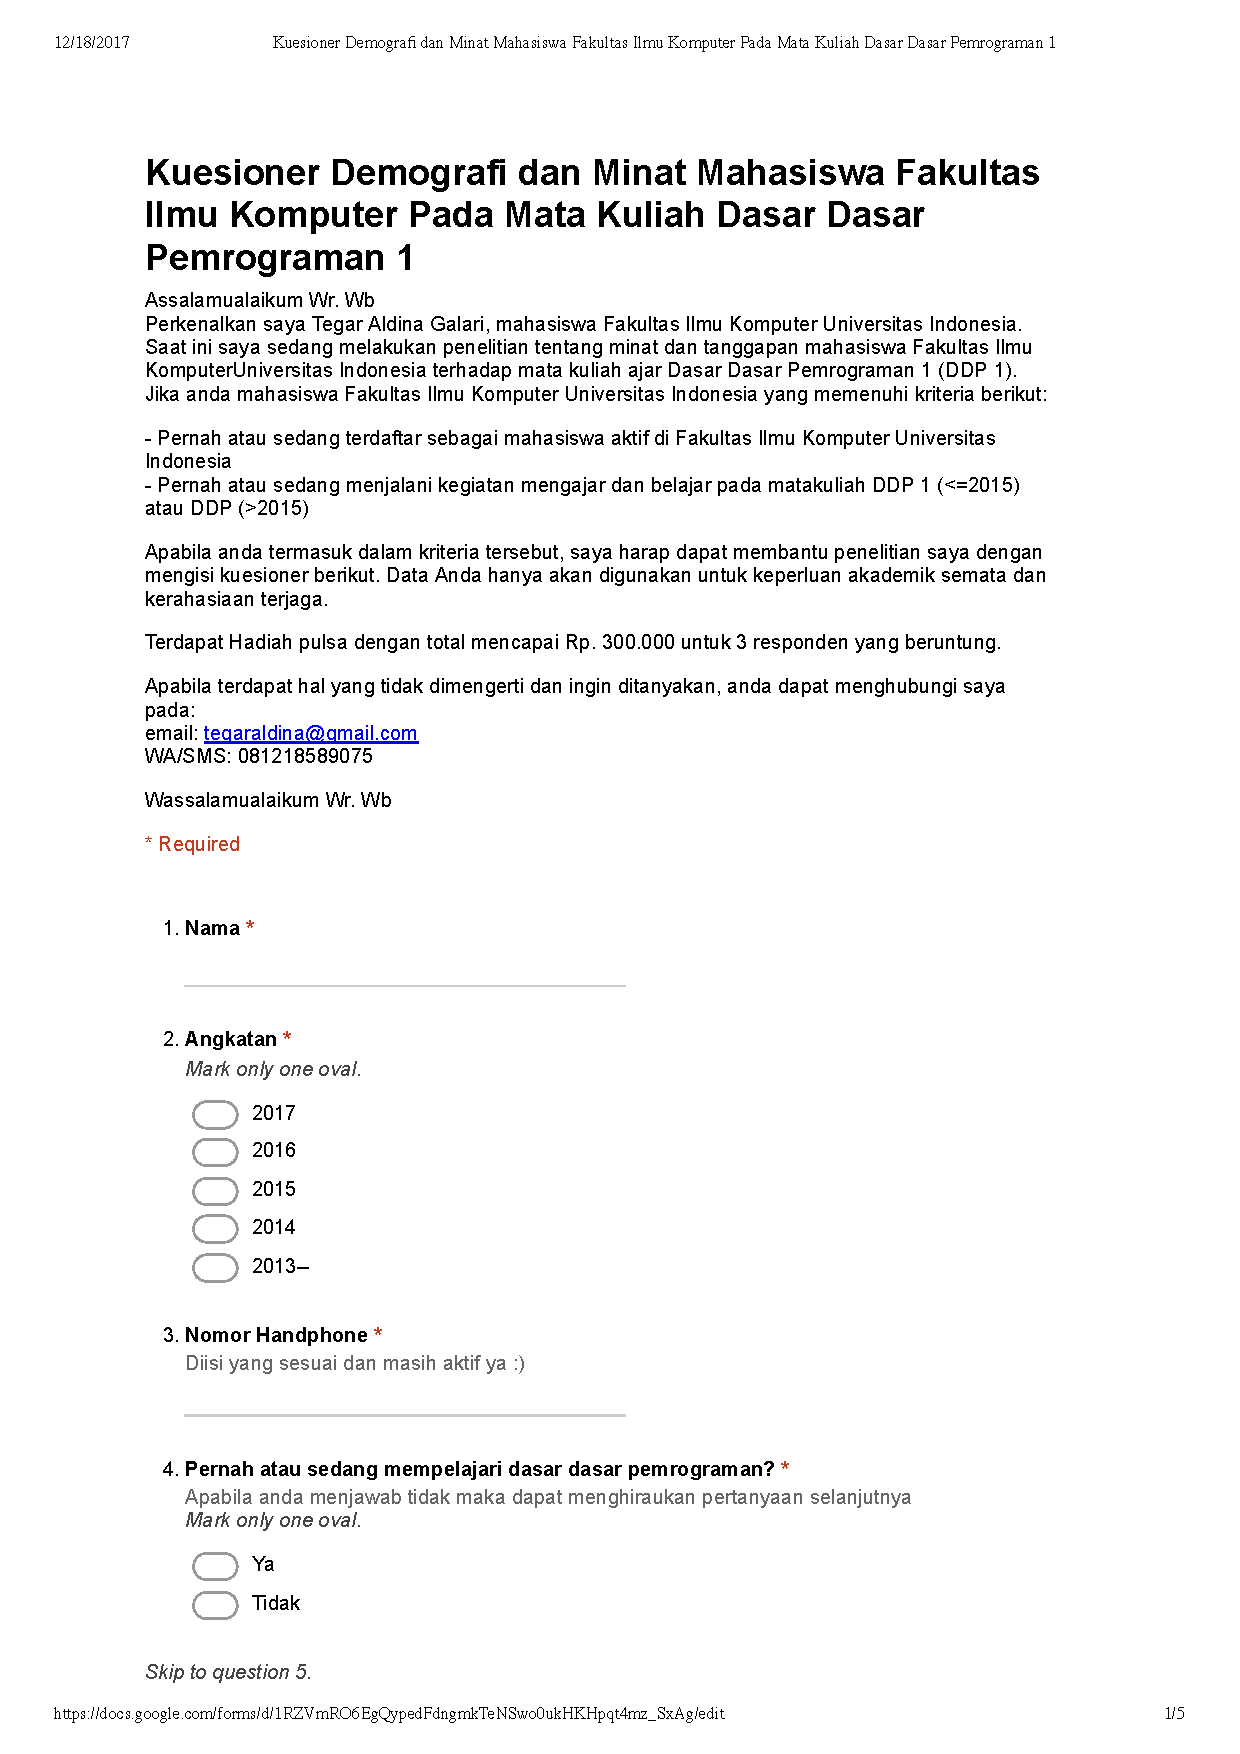
\includepdf[pages=-,pagecommand={},scale=0.6]{lampiran/Kuesoner-online.pdf}
%\end{longtable}

%-----------------------------------------------------------------------------%
\addChapter{Lampiran 2 : \textit{Form Usability Testing}}
\chapter*{Lampiran 2 : \textit{Form Usability Testing}}
%-----------------------------------------------------------------------------%
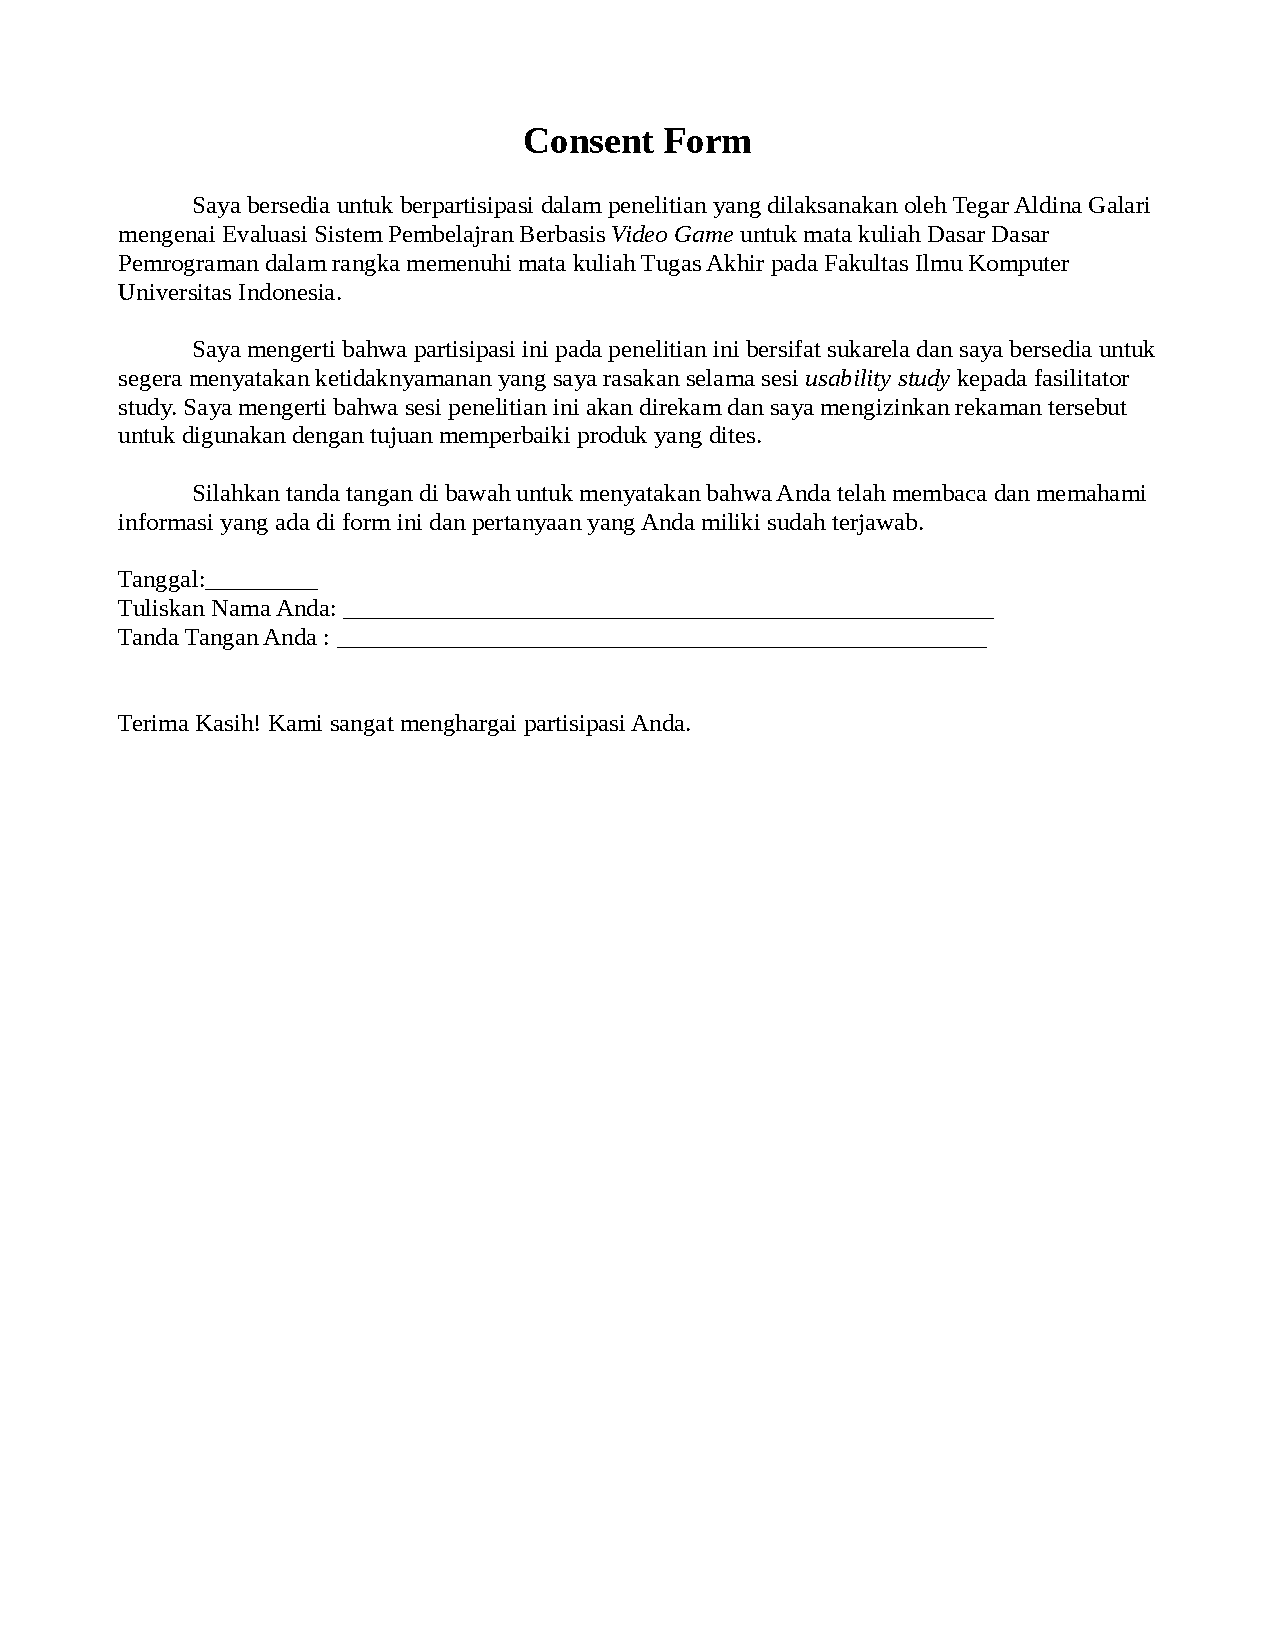
\includepdf[pages=-,pagecommand={},scale=0.9]{lampiran/form_UT.pdf}

\addChapter{Lampiran 3 : Hasil \textit{Usability Testing}}
%-----------------------------------------------------------------------------%
\begin{landscape}
	\chapter*{Lampiran 3 : Hasil \textit{Usability Testing}}
	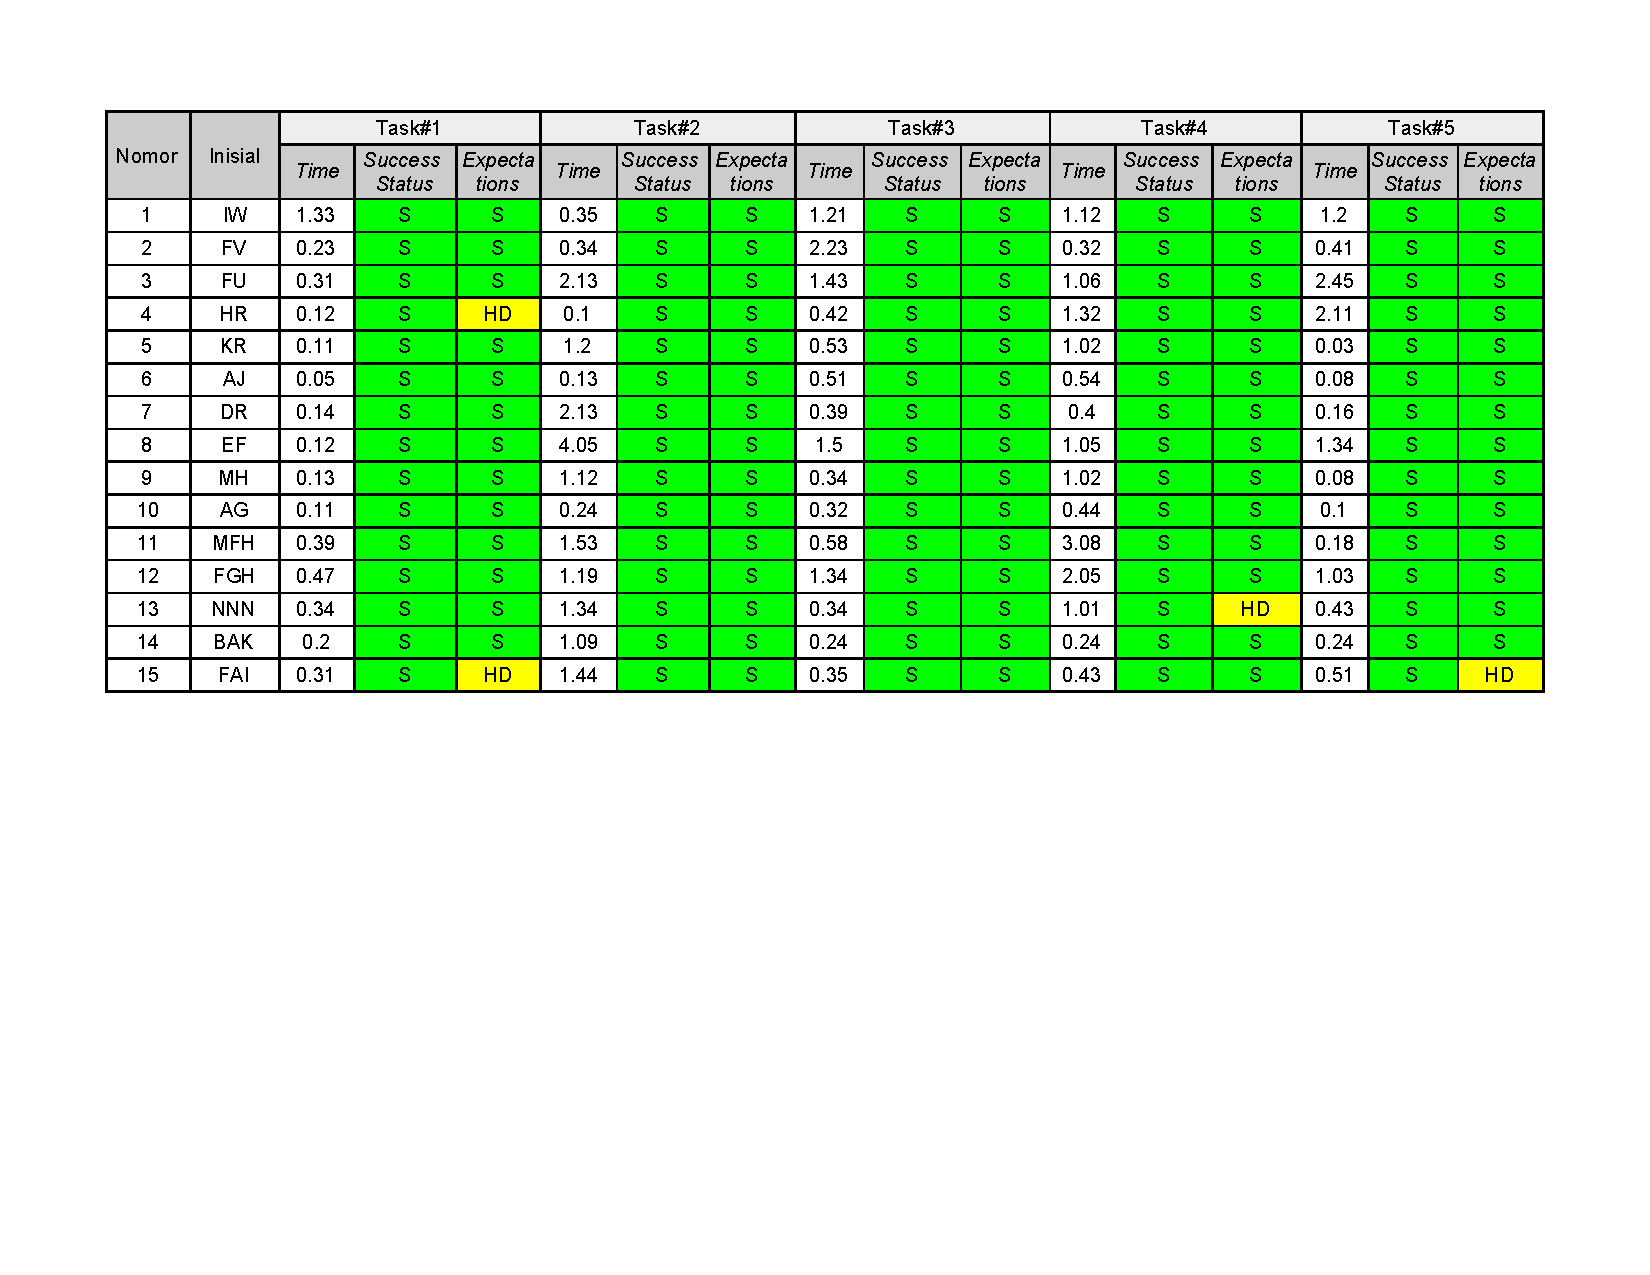
\includepdf[pages=-,pagecommand={},scale=1,angle=90]{lampiran/hasil-UT.pdf}
\end{landscape}

\end{appendix}

\end{document}